\documentclass[hyp,a4paper,12pt,openbib]{socreport}


\usepackage{fullpage}
\usepackage{tikz}
\usepackage{tikz-qtree}
\usepackage{tikz-qtree-compat}
\usepackage{amsmath,amsfonts}
\usepackage{caption, subcaption}
\usepackage{cancel, enumitem}
\usepackage{tabularx, array, amsmath, enumitem}

\usepackage{float}
\usepackage{pgfplotstable}

\usepackage{amsthm}

%\usepackage{hyperref}

\usepackage[capitalise]{cleveref}

\pgfplotsset{width=1\textwidth,compat=1.8, every axis/.append style={legend style = {legend pos=north west, ,font=\small, draw=none}, cycle list name=black white, legend cell align=left, font = \small, log basis x=2, log basis y=2, cycle list name=black white, width=1\linewidth}}
\usetikzlibrary{decorations.pathreplacing, arrows,positioning,calc,external}
\makeatletter \g@addto@macro\@floatboxreset\centering \makeatother
\renewcommand{\arraystretch}{1.2}


%\setcounter{secnumdepth}{4}
%\tikzexternalize

\newtheorem{lemma}{Lemma}
\newtheorem{theorem}{Theorem}


\begin{document}
\pagenumbering{roman}
\title{Efficient Key Aggregation for Cloud Storage}
\author{Chong Yun Long}
\projyear{2013/14}
\projnumber{H004900}
\advisor{Assoc. Prof. Chang Ee-Chien}
\deliverables{
	\item Report: 1 Volume}
	%\item Source Code: 1 DVD}		
\maketitle
\begin{abstract}
%There is a growing trend of outsourcing data storage to the cloud.  To protect 
%data confidentiality from the potentially curious public cloud servers, 
%it is desired to encrypt the data stored in the cloud, and issues 
%the decryption keys as and when needed.
%This give rise to a technical  issue on keys management,  as the distribution 
%could incur  substantial  overhead in storage, bandwidth and computation costs. 
%In this project, we look at such issues for  time-series data, for 
%e.g. video survillance data.   We consider a few known techniques, in particular,
%key-aggregation, ABE, and GGM. Although some of these technqies achieve 
%?..  We give a modification of KAC so as to reduce the public key size to constant?..

%Increasingly, organizations are outsourcing data storage to cloud services. As data is stores in remote servers, client-side encryption can be used to ensure data confidentiality. However, this also means that organizations have the additional responsibility of managing an inventory of keys. Storing and distributing these keys can incur substantial storage, bandwidth and computation costs, particularly in time-series data such as video files. By encrypting each video frame under different keys, decryption keys for each frame can be distributed independent of each other. This gives key granter the flexibility to vary access to specific portions of the video by releasing keys only for the relevant video frames, while preserving the confidentiality of frames which does not belong to the specified portions. In this project, we have devised a key management scheme that minimizes bandwidth as well as private storage required for distribution and inventory. The proposed scheme is also computationally efficient for the decryption of large sets of time-series data such as multimedia data.

%Increasingly, organizations are outsourcing data storage functions to cloud services. As data is stored in remote servers for cloud services, client-side encryption can be used to ensure data confidentiality. However, this also means that organizations have the additional responsibility of managing an inventory of keys for encryption. In addition, storing and distributing these keys can incur substantial storage, bandwidth and computation costs, particularly in time-series data such as video files. To tackle these issues, we have devised a key management scheme that minimizes bandwidth as well as private storage required for distribution and inventory. The proposed scheme is also computationally efficient for the decryption of large sets of time-series data such as multimedia data. (Transferred from end of para for flow from problem description to proposed solution) By encrypting each video frame under different keys, decryption keys for each frame can be distributed independent of each other. This gives key granters the flexibility to vary access to specific portions of the video by releasing only the decryption keys for the relevant video frames. Furthermore, The confidentiality of frames outside of the specific portion is preserved. 

%There is a growing trend of outsourcing data storage to the cloud.  To protect 
%data confidentiality from the potentially curious public cloud servers, 
%it is desired to encrypt the data stored in the cloud, and issues 
%the decryption keys as and when needed.
%This give rise to a technical  issue on keys management,  as the distribution 
%could incur  substantial  overhead in storage, bandwidth and computation costs. 
%In this project, we look at such issues for  time-series data, for 
%e.g. video survillance data.   We consider a few known techniques, in particular,
%key-aggregation, ABE, and GGM. Although some of these technqies achieve 
%?..  We give a modification of KAC so as to reduce the public key size to constant?..

Data storage outsourcing to public cloud services is a growing trend among organizations. To preserve data confidentiality from potentially curious cloud providers, organizations may choose to employ client-side encryption for data stored in the cloud. The keys are kept by the organization and are issued as and when required. However, this gives rise to technical challenges, as key storage and distribution can incur substantial storage, bandwidth and computational costs. In this project, we examine these issues for time-series data, e.g. video surveillance data. To address these issues, various known cryptographic techniques such as GGM tree, key-aggregate cryptosystem (KAC), attribute-based encryption (ABE) and multi-dimensional range query over encrypted data (MRQED) are considered. We propose a key management scheme which requires $O(1)$ private storage overhead and $O(\log^2(n))$ contiguous key-generation time. Furthermore, the scheme supports the distribution of keys for varying video frame rates and video resolution. These objectives are achieved through the use of GGM-KAC hybrid structures, homomorphic signature schemes, as well as modifications to KAC.

\begin{descriptors}
    \item E.3 Data Encryption
\end{descriptors}
\begin{keywords}
	applied cryptography, range query, multimedia encryption, attribute-based encryption, key aggregation
\end{keywords}

\begin{implement}
	Macbook Air 2013 (Intel Core-i7-4650u), Mac OS v10.9.2, Python 2.7.5, Charm v0.43
\end{implement}

\end{abstract}

\begin{acknowledgement}
   I would like to thank my advisor Assoc. Prof. Chang Ee-Chien for his guidance and inputs throughout the project. I would also like to express my appreciation to Miss Zhu Xiaolu, Mr Zhang Chunwang, Mr. Fang Chengfang for providing me with valuable feedback and advice.  \end{acknowledgement}

\listoffigures 
\listoftables
\tableofcontents 

\chapter{Introduction}

\label{chap:1}
With more and more organizations outsourcing data storage functions to cloud providers, the security and confidentiality of data in remote servers managed by third party have become a huge concern~\cite{kamara2010cryptographic}. Many providers such as Dropbox\footnote{https://www.dropbox.com/} and Google Cloud Storage\footnote{https://cloud.google.com/products/cloud-storage} encrypt data using server-side encryption where keys are managed by cloud providers. As these service providers have possession of the keys, they can easily access any data stored on their platforms, potentially compromising data confidentiality. Moreover, since authentication and access controls are enforced by public servers, there is a possibility of unauthorized users gaining access to the data. Distribution of data across multiple servers for redundancy further exacerbates the risk of data leakage. In view of all these complications, there is a huge incentive for users to perform client-side encryption before uploading their data onto an external cloud server. 

%With more and more organizations outsourcing data storage functions to cloud (server) providers, the security and con-fidentiality of data in  remote servers managed by third-parties have become a huge con-cern (Kamara  & Lauter, 2010). Many providers such as Dropbox 1 and Google Cloud Storage 2 encrypt data using server-side encryption where the keys are managed by providers of remote cloud servers. As these providers have possession of the keys, they can easily access any data stored on their platform, thus compromising data confidentiality. Moreover, since authentication and access controls are enforced by public servers, there is a possibility of unauthorized users gain-ing access to the data. Furthermore, cloud providers are also likely to distribute data across multiple servers for data redundancy, increasing the risk of data leakage. In view of all these complications, there is a huge incentive for users to perform client-side encryption before uploading their data onto an unsecured cloud server.

\section{Problem and Motivation}
\label{chap:1.1}
Although client-side encryption presents a possible solution to some of the security problems associated with cloud storage, accessing and sharing of encrypted data comes with its own set of unique problems and challenges. We shall illustrate some of these problems with an example.

Alice decides to upload her personal video onto the cloud to free up valuable storage on her SSD. However, she does not trust the cloud server with her data for fears of possible data leakage, preferring to encrypt the video with her own key before uploading. To view the videos, Alice simply retrieves the video from the cloud and decrypts the video using her own key. Bob, a friend of Alice requests for permission to view the video. Alice grants Bob access to her video by sending her key to Bob via a secured channel. Bob downloads the encrypted video from the cloud and decrypts it using the keys he had gotten from Alice.

Suppose the length of the video is 50 minutes, and Alice wants to restrict Bob to only the last 20 minutes of the video. Hence, Bob must not be able to decrypt the first 30 minutes of the video. In this scenario, the previous scheme will not work if the entire video is encrypted with only 1 key. With just 1 key, Bob is able to decrypt the entire video, and Alice would have inadvertently granted Bob access to the first 30 minutes of the video. To overcome this problem, Alice encrypts each video frame with distinct keys and transfers the keys for the last 20 minutes of the video to Bob via a secured channel. Under this simple scheme, the number of keys Alice has to share with Bob is linearly proportional to the length of video. For a 20 min, 24 FPS video, Alice will have to share $24 \times 60 \times 20 = 28800$ keys with Bob. Such a large key size could pose a problem in a channel with limited network bandwidth.

%Now suppose the length of the video is 50 minutes and that Alice only wants Bob to view the last 20 minutes, while keeping the first 30 minutes hidden from Bob. In this case, the previous scheme will not work if the entire video is encrypted with only 1 key since he can decrypt the entire video. This inadvertently gives him unauthorized access to the first 30 minutes of the video.

There are a variety of techniques that can be employed to reduce the size of key which Alice has to send to Bob. Some of these techniques require extra storage, while some others require extra computational power. The above example has illustrated a few important considerations:

\paragraph{Bandwidth} The total keysize that Alice needs to transfer to Bob should be small.
\paragraph{Storage} The total size of encryption keys that Alice has to store should be small. 
\paragraph{Runtime} Bob should not take a long time to decrypt the video frames.
\paragraph{Principle of least privilege} Bob only has access to the last 20 minutes of the video. Hence, the first 30 minutes of the video must not be revealed to Bob.
\paragraph{Collusion-resistant} Suppose Charles is also granted decryption keys to the same video. Bob and Charles should not be able to collude to decrypt video frames that neither of them can decrypt.
\paragraph{Expressiveness} Alice should have the flexibility to restrict Bob's access to the video to either a single frame or a set of frames. Similarly, Bob should have the flexibility to request for decryption keys to either a single frame or a set of frames. 
\section{Objective}

%first part is not clear. Such that the key granter can give a short key. Alice 

Alice faces a problem of large key size each time she shares keys with Bob. To solve Alice's problem, we want to devise a cryptographic and key management scheme that reduces the keysize needed for sharing of encrypted data. In this project, we will be focusing our efforts on multimedia data. The proposed scheme should also balance size of keys transferred with encryption/decryption time and storage overhead. Bob should not need to wait for hours to decrypt the video he got from Alice. Also, the ciphertext produced should not be significantly larger than plaintext.

\section{Contributions}
%We consider a model comprising of various entities. These entities are \textbf{Public Cloud (RC)}, \textbf{Key Granter (KG)}, \textbf{Data Owner (DO)} and \textbf{Authorized User (AU)}. With reference to this model, we have made the following contributions in this project:
We have made the following contributions in this project:


\begin{itemize}
%\item Proposed a model which comprising of various entities. These entities are \textbf{Public Cloud (RC)}, \textbf{Key Granter (KG)}, \textbf{Data Owner (DO)} and \textbf{Authorized User (AU)}.
\item Explored several existing techniques such as GGM construction, attribute-based encryption (ABE), Multi-dimensional Range Query over Encrypted Data (MRQED) and key-aggregate cryptosystem (KAC). We have also built prototypes to compare the empirical performance of ABE and KAC.
\item Developed a hybrid KAC-GGM scheme that is able to support contiguous decryption in $\log^2(n)$ time.
\item Observed that the runtime complexity of KAC decryption can be reduced from quadratic time to linear time for arithmetic sequences through the reuse of computed intermediate values. 
\item Developed a homomorphic MAC scheme that reduces storage requirements of key granter from $\Theta(n)$ to $O(1)$. 
\item Developed an encryption scheme which makes use of symmetric encryption to support fast decryption of layered content.
\end{itemize}




%contributions at start straight away give point form
%propose a model
%look at few existing schemes, and compare their performance
%hybrid of ggm of kac
%homorphics mac to reduce
%observations that kac is done faster in linear time

%modification of kac, reduce public size
%Although there are many existing schemes which are able to dramatically reduce the keysize, majority of them uses public-key cryptography together with bilinear pairings (discussed in \cref{sec:bilinear}) which may be too slow to be used for large data sets. These schemes may also produce ciphertext whose size is significantly larger than that of their plaintext equivalent. By using a combination of various algorithms and techniques, we have developed a key aggregation scheme which is efficient in runtime, storage overheads and bandwidth required for key distribution.


%By exploiting user access patterns and spatial organizations that are unique to multimedia data, as well as adopting some of the techniques from various existing schemes, we hope to produce a scheme that is efficient on large sets of multimedia data. We will also compare and evaluate our proposed scheme against some of these existing schemes.


%Multi-dimensional data is of special research interest because it serves as a good model for large data sets or Big Data. The emerging phenomena of Big Data meant that schemes which support such capabilities would be indispensable in the future. To this end, various existed cryptographic schemes will be evaluated and an in-depth analysis of each of the schemes will be presented.  Various metrics will be taken into consideration such as network bandwidth, storage space and computation time.

\chapter{Related work}

In this chapter, we examine related cryptographic schemes and evaluate how these schemes could be used as a possible solution to achieve our objectives. In \cref{sec:ggm}, we will explore the use of GGM trees as a possible solution to reduce key size. \cref{sec:abe} introduces ABE, a system which makes use of user attributes and access policies to manage ciphertext and keys. In \cref{chapt:mrqed}, we evaluate MRQED, a scheme that is used for encryption of multi-dimensional data. Finally, we present KAC in \cref{chap:kac}, a cryptosystem that is capable to aggregate any set of keys into a constant-size aggregate key. Many of these schemes are based on the use of bilinear pairings, a cryptographic operation which will be discussed in \cref{sec:bilinear}. 
%look at attribute-based. There are a few related techniques. Overview.

\section{GGM Tree}
\label{sec:ggm}
GGM Trees \cite{Goldreich1986} are used to generate pseudorandom numbers, or in our case encryption/decryption keys.

\subsection{GGM Construction}
Let $G$ be a cryptographically strong pseudorandom bit generator (CSB) that stretches a $s$-bits long input into a $2s$-bits long output. Denote $G_0$ to be the first $k$ bits and $G_1$ to be the last $k$ bits of the output from $G$.
$$G: \{0, 1\}^s \rightarrow \{0, 1\}^{2s}, G(x) = G_0(x) \, || \, G_1(x)$$

%In implementation, $G_1(x) = \text{SHA}_{256}(x \, || \, 'l' \, || \, \text{padding})$, $G_2(x) = \text{SHA}_{256}(x \, || \, 'r' \, || \, \text{padding})$.

Given seed $x$, we are able to construct a GGM tree with the root node, left child and right child represented by $x, G_0(x), G_1(x)$ respectively. \cref{fig:hash-tree} shows a GGM tree with $4$ leaf nodes. The security property of the CSB ensures that it is difficult to derive the right subtree using the left subtree and vice-versa.

%\begin{figure}[h]
%\centering
%\begin{tikzpicture}
% % all changes only affect trees within this environment
%\tikzset{level distance=50pt}
%\Tree [ .{$x$}
%[.{$G_l(x)$} [.{$G_l(G_l(x))$}    ]
%[ .{$G_r(G_l(x))$}   ] ]
%[.{$G_r(x)$} [.{$G_r(G_l(x))$}  ]
%[.{$G_r(G_r(x))$}  ] ] ]
%\end{tikzpicture}
%\caption{GGM tree}
%\label{fig:hash-tree}
%\end{figure}


\begin{figure}[ht]
\begin{minipage}[b]{0.5\textwidth}
\centering
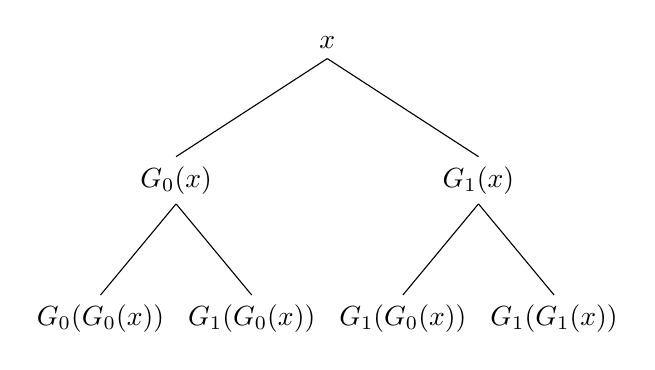
\begin{tikzpicture}
 % all changes only affect trees within this environment
\tikzset{level distance=50pt}
\Tree [ .{$x$}
[.{$G_0(x)$} [.{$G_0(G_0(x))$}    ]
[ .{$G_1(G_0(x))$}   ] ]
[.{$G_1(x)$} [.{$G_1(G_0(x))$}  ]
[.{$G_1(G_1(x))$}  ] ] ]
\end{tikzpicture}
\caption{GGM tree}
\label{fig:hash-tree}
\end{minipage}~
\begin{minipage}[b]{0.5\textwidth}
\centering
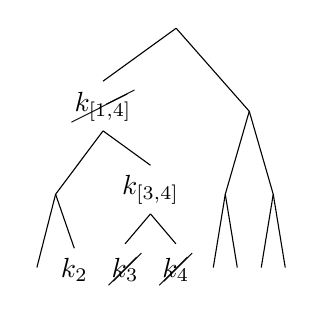
\begin{tikzpicture}
 % all changes only affect trees within this environment
%\tikzset{grow'=right} % make trees grow from left to right
%\tikzset{every tree node/.style={anchor=base west}} % allign nodes of the tree to the left (west)
\tikzset{frontier/.style={distance from root=120pt}}
\tikzset{level distance=30pt}
\Tree [ 
[.$\cancel{k_{[1,4]}}$  [ [.{} ] [.$k_2$ ]  ]
[ .$k_{[3,4]}$ [.$\cancel{k_3}$  ] [.$\cancel{k_4}$  ] ] ]
[  [ [.{}   ] [.{}  ] ]
[  [.{}   ] [.{}   ] ] ] ]
\end{tikzpicture}
\caption{Releasing keys for $[2, 4]$}
\label{fig:cover-ggm}
\end{minipage}
\end{figure}


The leaf nodes of the GGM tree can be used as encryption keys for the video frames (frame keys). To release the frame keys to Bob, Alice can aggregate the leaf nodes under their parent nodes, reducing the number of nodes Alice needs to transfer to Bob. We use $[x,y]$ to denote frames x to y inclusive.\footnote{$[x,y] = \{x,x + 1,...,y\}$}

%Since the root node can be used to derive subtrees, only a small storage footprint is required for the GGM tree. Only seed $x$ have to be stored in KG. Likewise, KG only have to send the seed to DO in order for DO to derive the decryption keys in the leaf nodes. The bandwidth required is only $O(1)$. 



%\begin{figure}[h]
%\centering
%\begin{tikzpicture}
% % all changes only affect trees within this environment
%%\tikzset{grow'=right} % make trees grow from left to right
%%\tikzset{every tree node/.style={anchor=base west}} % allign nodes of the tree to the left (west)
%\tikzset{frontier/.style={distance from root=120pt}}
%\tikzset{level distance=30pt,sibling distance=10pt}
%\Tree [ 
%[.$\cancel{k_{[1,4]}}$  [ [.{} ] [.$k_2$ ]  ]
%[ .$k_{[3,4]}$ [.$\cancel{k_3}$  ] [.$\cancel{k_4}$  ] ] ]
%[  [ [.{}   ] [.{}  ] ]
%[  [.{}   ] [.{}   ] ] ] ]
%\end{tikzpicture}
%\caption{Minimum number of keys for $[2, 4]$}
%\label{fig:cover-ggm}
%\end{figure}

In \cref{fig:cover-ggm}, Alice just needs to send nodes $\{k_2, k_{[3,4]}\}$ for Bob to obtain the keys for $[2,4]$. However, Alice cannot send Bob $k_{[1,4]}$ because Bob is able to derive $k_{1}$, thus allowing him to decrypt frame $1$ which he is not entitled to have access to. Alternatively, Alice could also choose to send $\{k_2, k_3, k_4\}$ to Bob. However, this is less efficient than sending Bob $\{k_2, k_{[3,4]}\}$.

\subsection{Evaluation}

Alice only have to send Bob a logarithmic-size key for contiguous range queries\footnote{Queries in the form $[x,y]$}.
However, non-contiguous queries can yield a worst-case keysize of $O(n)$ where $n$ is the total number of frames in the video. This can occurs if the requested frame keys follows an arithmetic sequence, $a_i = a_1 + (i-1)d$, where $d \geq 0$ and $i$ being the frame number ($i\geq 1$). In this situation, none of the frame keys requested can be aggregated under a common parent node. For example, consider the case where Bob request for keys to all the odd frames. Consequently, the requested frames can be expressed as an arithmetic sequence of the form $a_i = 1 + 2(i-1)$. Since none of the frames can be aggregated, Alice needs to send $n/2$ leaf nodes to Bob.

Alice does not have to store all of the frame keys as she can derive the frame keys from the root node, albeit at the cost of increased computational time. As a result, storage overhead is reduced from $\Theta(n)$ to $O(1)$. 

\section{Attribute-Based Encryption}
\label{sec:abe}
Attribute-Based Encryption (ABE)~\cite{bethencourt2007ciphertext,waters2011ciphertext,goyal2006attribute,sahai2005fuzzy,lewko2010revocation} is a scheme where the ciphertext and the corresponding keys are dependent on attributes and access structures. Depending on the type of access policy, ABE can be classified broadly into two catgories, namely cipertext-policy ABE~\cite{bethencourt2007ciphertext,waters2011ciphertext} and key-policy ABE~\cite{goyal2006attribute,lewko2010revocation}. 


%ABE can be classified into either ciphertext-policy~\cite{bethencourt2007ciphertext,waters2011ciphertext} or key-policy~\cite{goyal2006attribute,lewko2010revocation}. 

\subsection{Ciphertext-Policy ABE}
We introduce the notion of ciphertext-policy ABE (CP-ABE) with a simple example. Alice wants to share a video with her mother, father, brother, her classmates of class 4C (year 4, class C) as well as her female choir friends. In CP-ABE, each key that a user possesses will be associated with a set of descriptive attributes. The attributes involved in this example are \texttt{mother}, \texttt{father}, \texttt{brother}, \texttt{year 4}, \texttt{class C}, \texttt{choir}, \texttt{female} and  \texttt{male}. Alice's mother's key will be encrypted with the attribute set $\{\texttt{mother, female}\}$, represented by $K_{\{\texttt{mother, female}\}}$. 

The criterion needed to decrypt the video is termed as an ``access policy''. We represent access policy with a boolean formula involving \textbf{AND} and \textbf{OR} gates. In this example, Alice is able to specify the video's access structure as: (\texttt{mother} \textbf{OR} \texttt{father} \textbf{OR} \texttt{brother} \textbf{OR} (\texttt{year 4} \textbf{AND} \texttt{class C}) \textbf{OR} (\texttt{female} \textbf{AND} \texttt{choir})). The boolean formula is then transformed into a policy tree as shown in \cref{fig:access-tree}. The attributes form the leaves of the access tree while the \textbf{AND} and \textbf{OR} gates form the inner nodes. 


\begin{figure}[h]
\centering
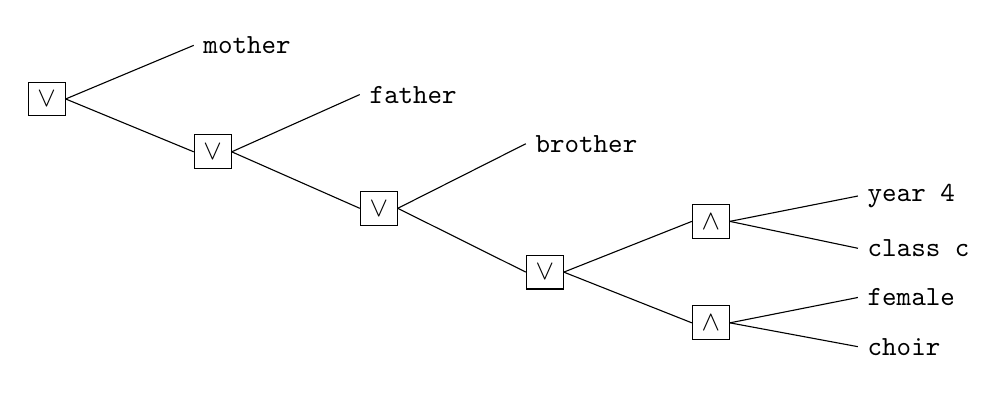
\begin{tikzpicture} % all changes only affect trees within this environment
\tikzset{grow'=right} % make trees grow from left to right
\tikzset{every tree node/.style={anchor=base west}} % allign nodes of the tree to the left (west)
\tikzset{level distance=60pt,sibling distance=5pt}
\Tree [.\node[draw, rectangle]{$\vee$}; [.\texttt{mother} ][. \node[draw, rectangle]{$\vee$}; [.\texttt{father} ][.\node[draw, rectangle]{$\vee$}; [.\texttt{brother} ] [.\node[draw, rectangle]{$\vee$}; [.\node[draw, rectangle]{$\wedge$};  [.\texttt{year 4} ]   [.\texttt{class c} ] ]   [.\node[draw, rectangle]{$\wedge$}; [.\texttt{female} ][. \texttt{choir} ] ]]  ] ]  ] 
\end{tikzpicture}
\caption{Access Tree with \textbf{AND}, \textbf{OR} gates} \label{fig:access-tree}
\end{figure}


As a generalization of ABE, we are able to replace \textbf{AND} and \textbf{OR} nodes with threshold gates shown in \cref{fig:access-tree-thresh}. For instance, a 2/5 threshold gate is evaluated to true only if any 2 out of 5 subtrees of the threshold gate are evaluated to be true. As a generalization, an \textbf{AND} gate can be represented by a 2/2 gate and an \textbf{OR} gate can be represented by a 1/2 gate.

\begin{figure}[h]
\centering
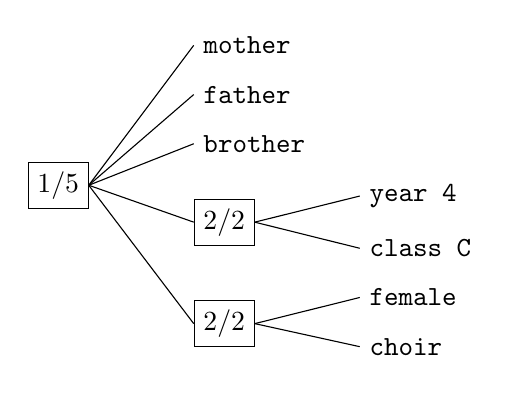
\begin{tikzpicture} % all changes only affect trees within this environment
\tikzset{grow'=right} % make trees grow from left to right
\tikzset{every tree node/.style={anchor=base west}} % allign nodes of the tree to the left (west)
\tikzset{level distance=60pt,sibling distance=5pt}
\Tree [.\node[draw, rectangle]{$1/5$}; [.\texttt{mother}  ] [.\texttt{father} ] [.\texttt{brother} ] [.\node[draw, rectangle]{$2/2$}; [.\texttt{year 4} ] [.\texttt{class C} ] ]   [.\node[draw, rectangle]{$2/2$}; [.\texttt{female} ] [.\texttt{choir} ] ]  ] 
\end{tikzpicture}
\caption{Access Tree with threshold gates} \label{fig:access-tree-thresh}
\end{figure}

Using the same example, we consider Bob who is in the same year and same choir as Alice and Charles who is Alice's classmate. Correspondingly, Bob receives $K_{\{ \text{year 4, male, choir}\} }$ while Charles receives $K_{\{ \text{year 4, class C, male}\} }$. Bob is unable to decrypt the video because he neither satisfies the female\footnote{The \texttt{male} attribute is not represented in the access tree} choir member criteria nor the class c criteria. In contrast, the access tree evaluates to be true with respect to attribute set $\{ \texttt{year 4}, \texttt{class C}\}$. Since, $\{ \texttt{year 4}, \texttt{class C}\} \subset \{ \texttt{year 4, class C, male}\}$, Charles in possession of $K_{\{ \text{year 4, class C, male}\} }$ is able to decrypt the video. In CP-ABE, the access policy is associated with ciphertext and the attributes are associated with the keys, hence the name ``ciphertext-policy''.



%Charles is granted access because access tree evaluates to true with attribute set \{\texttt{year 4}, \texttt{class C}\}, which is a subset of . 

\subsection{Key-Policy ABE}

In KP-ABE, the access policy is associated with keys and the attributes are associated with the ciphertext, hence the name ``key-policy''. We reference to the example discussed in \cref{chap:1.1}. Instead of sending a distinct key for each frame, Alice uses KP-ABE to encrypt each video frame with the frame number as its attribute. For a video with $n$ frames, Alice can issue to Bob $K_{\{ (n-28799) \vee (n-28798) \vee \dots \vee n) \}}$. The access policy in this case is a series of \textbf{OR} gates for every frame in the last 20 minutes of the video. Bob will thus be able to decrypt all frames in the range $[n-28799, n]$. However, the key transmitted is still linear in size. An algorithm that represents contiguous sets more efficiently\footnote{It is possible to represent $[n-28799, n]$ using logarithmic number of attributes} will be introduced in \cref{sec:abe-range}.


%\begin{figure}[h] [. $\vee$  [.\texttt{class c} ] [. $\wedge$ [.\texttt{female} ][. \texttt{choir} ]]]
%\begin{tikzpicture} % all changes only affect trees within this environment
%\tikzset{grow'=right} % make trees grow from left to right
%\tikzset{every tree node/.style={anchor=base west}} % allign nodes of the tree to the left (west)
%\tikzset{level distance=60pt,sibling distance=5pt}
%\Tree [.$\vee$ [.$\vee$ [ [.$\wedge$ [.\texttt{student-year>2}  ]  [.$\vee$ [.\texttt{"science"}  ] [.\texttt{"engineering"} ] ] ]   ] [.\texttt{"faculty staff"} ] ] [.$\wedge$ [.\texttt{"admin staff"}   ] [.\texttt{job-grade>4} ] ] ]
%\end{tikzpicture}
%\caption{Access Tree} \label{fig:access-tree}
%\end{figure}

%\begin{figure}[h]
%\centering
%\begin{tikzpicture} % all changes only affect trees within this environment
%\tikzset{grow'=right} % make trees grow from left to right
%\tikzset{every tree node/.style={anchor=base west}} % allign nodes of the tree to the left (west)
%\tikzset{level distance=70pt,sibling distance=5pt}
%\Tree [.$1/3$  [ [.$2/2$ [.\texttt{student-year>2}  ]  [.$1/2$ [.\texttt{"science"}  ] [.\texttt{"engineering"} ] ] ]   ] [\texttt{"faculty staff"} ]  [.$2/2$ [.\texttt{"admin staff"}   ] [.\texttt{job-grade>4} ] ] ]
%\end{tikzpicture}
%\caption{Access Tree with threshold gates} \label{fig:access-tree-thresh}
%\end{figure}

%Realization of ABE
\subsection{Realization of ABE}
In this section, we describe the algorithms used in KP-ABE. However, we will not discuss the details of KP-ABE construction in this report. The KP-ABE scheme in~\cite{lewko2010revocation} consists of 5 algorithms, as shown in~\cref{tab:kpabe-algo}.
%Let us look into the detailed schematics of ABE. We take also take a look at the protocol of CP-ABE.

%\subsubsection{KP-ABE in Detail}


%\begin{description}
%\item[Setup]  -- Output: Master Secret Key (\texttt{msk}), Public Key (\texttt{pk})
%\item[Encrypt] -- Inputs: \texttt{pk}, Message (\texttt{msg}), Access Structure ($\mathbb{A}$); Outputs: Ciphertext ($\mathfrak{C}$)
%\item[KeyGen] -- Inputs \texttt{msk}, Attribute set ($S$)\\
%Output: Secret key (\texttt{sk}) for set $S$
%\item[Decrypt] \hfill \\
%Input: $\mathfrak{C}$, \texttt{sk}
%Output: \texttt{msg} if $S$ satisfies $\mathbb{A}$
%\item[Delegate] \hfill \\
%Input: \texttt{sk}, Attribute set $\tilde{S}$ where $\tilde{S} \subseteq S$ \\
%Output: $\tilde{\texttt{sk}}$ for set $\tilde{S}$
%\end{description}

%\begin{table}[h]
%{\renewcommand{\arraystretch}{1.2} %<- modify value to suit your needs
%    \begin{tabular}{|l|l|l|}
%    \hline
%    \textbf{Algorithm} & \textbf{Inputs}                                                      & \textbf{Outputs}                                           \\ \hline
%    Setup              & --                                                                    & Master Secret Key (\texttt{msk}), Public Key (\texttt{pk}) \\ \hline
%    Encrypt            & \texttt{pk}, Message (\texttt{msg}), Access Structure ($\mathbb{A}$) & Ciphertext ($\mathfrak{C}$)                                   \\ \hline
%    KeyGen             & \texttt{msk}, Attribute set ($S$)                                    & Secret key (\texttt{sk}) for set $S$                       \\ \hline
%    Decrypt            & $\mathfrak{C}$, \texttt{sk}                                             & \texttt{msg} if $S$ satisfies $\mathbb{A}$                 \\ \hline
%    Delegate           & \texttt{sk}, Attribute set $\tilde{S}$ where $\tilde{S} \subseteq S$ 	& $\tilde{\texttt{sk}}$ for set $\tilde{S}$ \\ \hline
%    \end{tabular}
%}
%    \caption {CP-ABE Algorithms}
%\label{tab:cpabe-algo}
%\end{table}


\begin{table}[H]
\begin{tabular}{|l|p{0.4\textwidth}|p{0.3\textwidth}|}
    \hline
    \textbf{Algorithm} & \textbf{Inputs}                                           & \textbf{Outputs}                 \\ \hline
    \textbf{Setup}              & Generators $g,h$ \newline Exponents $a', a'', b \in \mathbb{Z}_p$ & Master Key (MK) \newline Public Key (PK) \\ \hline
    \textbf{Encryption}         & PK, Message ($M$), Attribute set ($\gamma$)               & Ciphertext ($E$)                 \\ \hline
    \textbf{Key Generation}     & MK, PK, Access structure ($\mathbb{A}$)                   & Private Key ($D$)                \\ \hline
    \textbf{Decryption}         & $E,D$                                                     & $M$                              \\ \hline
    \end{tabular}
    \caption {KP-ABE algorithms}
\label{tab:kpabe-algo}
\end{table}




It is easy to see how this scheme can be adapted to a cloud storage. Alice runs \textbf{Setup} and uses \textbf{Key Generation} together with access structure $\mathbb{A}$ specified for Bob, producing Bob's private key ($D$). Alice next encrypts $M$ (video frame) under attribute set $\gamma$ (frame number) and stores it on the cloud. Bob is then able to use $D$ to decrypt $M$ if $\gamma$ satisfies $\mathbb{A}$. Also, \textbf{Key Generation} randomizes the keys generated to prevent collusion, a situation where two different parties are able to combine their keys to decrypt messages that neither of them has access to. 


\subsection{ABE Operations and Structures}

In this section, we take a look at some of the operations and structures that are used in ABE.

 \subsection{Bilinear Map}
 \label{sec:bilinear}
Bilinear Map is a fundamental cryptographic operation used in ABE as well as many other encryption schemes. Let $\mathbb{G}_1, \mathbb{G}_2, \mathbb{G}_3$ be groups of prime order $p$, $u \in \mathbb{G}_1, v \in \mathbb{G}_2$.
A bilinear pairing $e:\mathbb{G}_1 \times \mathbb{G}_2 \to \mathbb{G}_3$  has the following properties:

\begin{description}
\item[Bilinearity] $a, b \in \mathbb{Z}_p, \, e(u^a, v^b) = e(u, v)^{ab}$
\item[Non-degeneracy] $e(u,v) \neq 1$
\item[Computable] $e$ can be computed efficiently for practical purposes.
\end{description}

\subsection{Monotonic Access Schemes}

Most ABE schemes are based on monotonic access schemes. Let $\mathbb{A} \subseteq 2^{\{P_1, P_2, \dots, P_n\}}$, where $\{P_1, P_2, \dots, P_n\}$ refer to the set of parties. A collection $\mathbb{A}$ is monotonic if $\forall B, C$, if $B\in \mathbb{A}$ and $B \subseteq C$ then $C\in \mathbb{A}$. An access structure is a collection $\mathbb{A}$ of non-empty subsets, that is $\mathbb{A} \subseteq 2^{\{P_1, P_2, \dots, P_n\}} \backslash \{\emptyset\}$. This means that we do not consider the unauthorized sets which are not in $\mathbb{A}$ An example of a non-monotonic policy would be ``students who do not belong to Alice's class''. One possible solution would be to represent negation as a separate attribute but this would result in a huge increase in the number of attributes required. There are however ABE schemes proposed which allow policies to be expressed in non-monotonic access structures~\cite{ostrovsky2007attribute}. For this project, we will not be considering non-monotonic access structures.

%
\subsection{Range Comparison}
\label{sec:abe-range}
Using ``bag of bits'' representation~\cite{bethencourt2007ciphertext}, we are able to support integer comparisons using $O(n)$ gates, for an $n$ bit integer. We represent 4 bit attribute such as ``$x=9$' using 4 attributes \{\texttt{x:1***}, \texttt{x:*0**}, \texttt{x:**0*}, \texttt{x:***1}\}. \textbf{AND}, \textbf{OR} gates is then used to implement comparisons such as ``$x<10$''  with a policy illustrated in \cref{fig:access-tree-range}.

\begin{figure}[h]
\centering
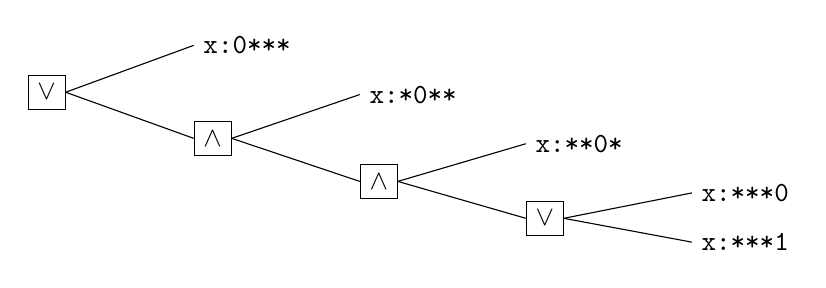
\begin{tikzpicture} % all changes only affect trees within this environment
\tikzset{grow'=right} % make trees grow from left to right
\tikzset{every tree node/.style={anchor=base west}} % allign nodes of the tree to the left (west)
\tikzset{level distance=60pt,sibling distance=5pt}
\Tree [.\node[draw, rectangle]{$\vee$}; [.\texttt{x:0***} ] [.\node[draw, rectangle]{$\wedge$}; [.\texttt{x:*0**} ]  [.\node[draw, rectangle]{$\wedge$}; [.\texttt{x:**0*}  ]   [.\node[draw, rectangle]{$\vee$};  [.\texttt{x:***0}  ]  [.\texttt{x:***1}  ]  ]  ]  ] ] ] 
\end{tikzpicture}
\caption{Policy tree for $x<10$} \label{fig:access-tree-range}
\end{figure}

It is easy to verify that ``$x=9$'' satisfies the policy tree. 4 bit integers which are larger than or equal to 10 such as ``$x=13$'' represented as \{\texttt{x:1***}, \texttt{x:*1**}, \texttt{x:**0*}, \texttt{x:***1}\}, is unable to satisfy the policy tree.
 
 


\subsection{Evaluation}
 
 
Since ABE's key and ciphertext size grow linearly with respect to the number of attributes, the ``bag of bits'' representation will result in a key and ciphertext size logarithmic to the value of the numerical attribute. Using KP-ABE, Alice would encrypt each video frame together with their respective frame number using the ``bag of bits'' representation. Alice then generates Bob's key restricting him to a specific range of frames. This is done again using the ``bag of bits'' representation. Using this method, Alice only has to send one single logarithmic-size key to Bob, resulting in a huge reduction in key size.

Depending on the number of attributes and type of access policies, ABE can be computationally expensive due to the pairing and exponentiation operations it has to perform. More investigations are needed to determine its efficiency for large datasets. 

\subsection{Multi-message Ciphertext Policy ABE}
\label{chapt:mcp-abe}
Multi-message Ciphertext Policy ABE or MCP-ABE~\cite{2013scalable} is a scheme that is built upon CP-ABE, catered specifically for scalable media. The paper proposed segmentation of media content into $l$ layers, each with different privilege rights. A video file for instance can be segmented into subtitles, audio, low quality video (LQ) and high quality video enhancement (HQ). Each of this layer is associated with an access privilege: $p_l, p_{l-1}, \dots ,p_1$, and $p_{i+1}$ having a higher privilege than $p_{i}$. The highest privilege level is $p_l$ while the lowest is $p_1$. Suppose that Alice has access to HQ enhance layer with the highest privilege $p_l$.  Alice should also have access to all other layers of lower privileges (subtitles, audio, low quality video). Hence, $p_l$ should grant access to the keys of not only $k_l$ but also all the other keys. This is accomplished through the use of a chain hash. 
\begin{equation}\label{eq:hash-chain}
k_j = H(k_{j+1}||j), j=l-1, \dots, 2, 1
\end{equation}

$k_l$ is hashed repeatedly to generate keys for all other layers. It is not computationally feasible to generate $k_{j+1}$ from $k_j$ due to preimage resistance of the cyptographic hash function. 

Unlike in CP-ABE where each access structure is associated with a single ciphertext message, MCP-ABE  associates multiple messages with a single policy tree as shown in \cref{fig:access-tree-mcp}. Each message is a symmetric key which is used for decryption of the respective layers. The keys are derived using the hash chain shown in Equation \ref{eq:hash-chain}. The ability to associate encrypt multiple messages using a single access tree allows us to have a hierarchy of access levels.
\begin{figure}[h]
\centering
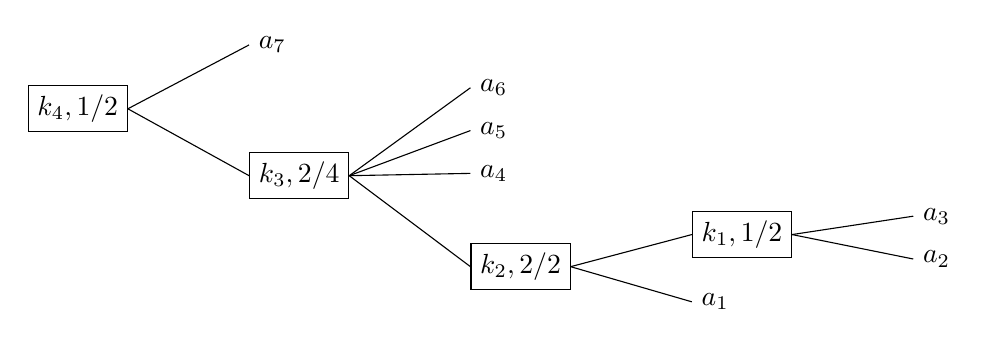
\begin{tikzpicture} % all changes only affect trees within this environment
\tikzset{grow'=right} % make trees grow from left to right
\tikzset{every tree node/.style={anchor=base west}} % allign nodes of the tree to the left (west)
\tikzset{every tree node/.style={anchor=base west}}
\tikzset{level distance=80pt,sibling distance=3pt}
\Tree [.\node[draw,rectangle]{$k_4,1/2$}; [.$a_7$ ]
[.\node[draw,rectangle]{$k_3,2/4$}; [.$a_6$  ] [.$a_5$ ] [.$a_4$ ]
[.\node[draw,rectangle]{$k_2,2/2$};
[.\node[draw,rectangle]{$k_1,1/2$}; [.$a_3$  ][.$a_2$  ]]
[.$a_1$ ] ] ] ]
\end{tikzpicture}
\caption{MCP-ABE access tree} \label{fig:access-tree-mcp}
\end{figure}

 Each threshold gate is associated with a particular message, which in this case is a symmetric key used for media decryption. Since the keys are generated via a hash chain, having $a_7$ would allow the user to calculate $k_4$. Using $k_4$, a user would be able to use Equation \ref{eq:hash-chain} to obtain all other keys ($k_3,k_2,k_1$). 

\section{Multi-dimensional Range Query over Encrypted Data}
\label{chapt:mrqed}

Suppose Alice organizes the frames belonging to different videos into a multi-dimensional scheme by tagging them with GPS latitude and longitudinal coordinates $(la, lo)$, timestamp ($t$) of the video, picture resolution ($p$) and frame number ($f$). Each video frame can be referenced by tuple $(la, lo, t, q, f)$. Multi-dimensional Range Query over Encrypted Data~\cite{shi2007multi,Bethencourt06anonymousmultiattribute}, or MRQED is a scheme that allows for small key sizes in the encryption and decryption of such multi-dimensional data.

MRQED organizes the public keys and private keys ($ID$) into interval trees, each node in charge of encrypting a particular range/point.


\begin{figure}[h]
 \begin{subfigure}{.63\textwidth}
 \centering
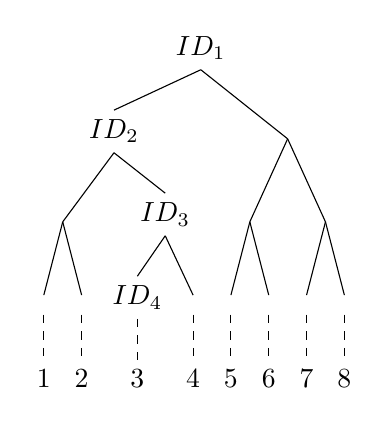
\begin{tikzpicture} % all changes only affect trees within this environment
%\tikzset{grow'=right} % make trees grow from left to right
%\tikzset{every tree node/.style={anchor=base west}} % allign nodes of the tree to the left (west)
\tikzset{frontier/.style={distance from root=120pt}}
\tikzset{level distance=30pt}
\Tree [.${ID_1}$ 
[.${ID_2}$  [ [.{} \edge[dashed]; {$1$}   ] [.{} \edge[dashed]; {$2$}  ]  ]
[.${ID_3}$  [.${ID_4}$ \edge[dashed]; {$3$} ] [.{} \edge[dashed]; {$4$}  ] ] ]
[  [ [.{} \edge[dashed]; {$5$}   ] [.{} \edge[dashed]; {$6$}    ] ]
[  [.{} \edge[dashed]; {$7$}   ] [.{} \edge[dashed]; {$8$}   ] ] ] ] 
\end{tikzpicture}
\caption{Encryption for frame $3$ under 4 different $ID$}
\label{fig:mrqed-encrypt}
\end{subfigure} \begin{subfigure}{.33\textwidth}
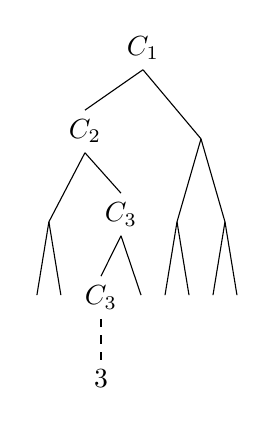
\begin{tikzpicture}
\Tree [.$C_1$ 
[.$C_2$  [ [.{} ] [.{}  ]  ]
[.$C_3$  [.$C_3$ \edge[dashed]; {$3$}  ] [.{} ] ] ]
[  [ [.{}  ] [.{}   ] ]
[  [.{} ] [.{} ] ] ] ]
\end{tikzpicture}
\caption{4 different ciphertexts for frame $3$}
\label{fig:mrqed-ciphertext}
\end{subfigure}

\caption{Encryption under MRQED}
\label{fig:mrqed}
\end{figure}%



In~\cref{fig:mrqed-encrypt}, Alice has to encrypt frame $3$ a total of 4 times under $\{ID_1, ID_2, ID_3, ID_4\}$ since all of these nodes covers frame $3$. As a result, 4 different ciphertexts will be produced for $f_3$ as shown in \cref{fig:mrqed-ciphertext}. Encryption of a single frame will take $O(\log(n))$ time. Each piece of ciphertext (a single encrypted frame) will occupy $O(\log(n))$ space. Keys are released in a manner similar to the GGM tree illustrated in \cref{fig:cover-ggm}. 

%Alice have encrypted all 8 video frames and uploaded them onto the cloud. Bob wishes to retrieve the range $[f_2, f_4]$.  In \cref{fig:cover2-4}, Alice just needs to send 2 keys $\{k_B, k_C\}$ for Bob to decrypt $[f_2, f_4]$. Since $k_c$ covers $[f_3,f_4]$ and $k_b$ covers $f_2$, $\{k_B, k_C\}$ will be sufficient for Bob to decrypt $[f_2, f_4]$   Alice cannot send Bob $k_A$ since it covers the range $[f_1, f_4]$, allowing Bob to decrypt $f_1$ which he is not entitled to have access to. Alice could also choose to send 3 keys, $\{k_B, k_D, k_E\}$ to Bob. However, doing so is lesser efficient than sending Bob $\{k_B, k_C\}$, which contains only 2 keys.
%

%
%\begin{figure}[h]
%\centering
%\begin{tikzpicture}
% % all changes only affect trees within this environment
%%\tikzset{grow'=right} % make trees grow from left to right
%%\tikzset{every tree node/.style={anchor=base west}} % allign nodes of the tree to the left (west)
%\tikzset{frontier/.style={distance from root=120pt}}
%\tikzset{level distance=30pt,sibling distance=10pt}
%\Tree [ 
%[.$\cancel{k_A}$  [ [.{} \edge[dashed]; {$f_1$} ] [.$k_B$ \edge[dashed]; {$f_2$} ]  ]
%[ .$k_C$ [.$\cancel{k_D}$ \edge[dashed]; {$f_3$} ] [.$\cancel{k_E}$ \edge[dashed]; {$f_4$}  ] ] ]
%[  [ [.{}   ] [.{}  ] ]
%[  [.{}   ] [.{}   ] ] ] ]
%\end{tikzpicture}
%\caption{Minimum number of keys for $[f_2, f_4]$}
%\label{fig:cover2-4}
%\end{figure}


%Even though $k_A$ covers $p=2$, it leaks information about $p=1$. $\{k_D, k_E$\} is not released because it is not the minimum cover. A single key ($k_C$) is sufficient to represent $[3,4]$. The key size is logarithmic, $O(\log(T))$ to the data range (number of leaves). Extending it to multi-dimensional data results in $O(D\log(T))$ key size. The range tree belonging to each separate dimension can be connected via an $\wedge$ gate.

%To release the decryption keys for $[a,b]$, we consider the minimum number of subtrees covering $[a,b]$. $\{k_B,k_C\}$ is released for $[2,4]$.

%To produce ciphertext for message $m$, $msg$ is encrypted under point $p=4$, $m$ is encrypted with the set of $IDs$ covering $p=4$. The set of $IDs$ is the collection of nodes from $p=4$ to the root.  It is not hard to see that the ciphertext is logarithmic in size, each node along the path from root to $p=4$ contains $C_i = Encrypt(PK, ID_i, m||0^{|m|})$. The appended $|m|$ trailing $0$s (denoted by $0^{|m|}$) serves as a message verification during decryption. 




% encrypted $log(T)$ times, $T$ being the total number of data points (leaf nodes). 



\subsection{MRQED for multiple dimensions}

MRQED can be extended to multiple dimensions. Intuitively, we build $D$ trees for $D$ dimensions. In \cref{fig:mrqed-alice}, Alice wants to release keys for $x1=[2,4], y1=[5,6]$ to Bob. To do so, we find a minimum cover for $x_1$ and release key set $k_{x1}$. Likewise for $y1$, we obtain the minimum cover key set $k_{y1}$. To decrypt hyperrange $\{x1,y1\}$ we send Bob $k_{x1}$ and $k_{y1}$. This is a very efficient construction, with a decryption key size of only $O(D\log(n))$ with no additional overhead.
\begin{figure}[h]
\begin{subfigure}[t]{.33\textwidth}
\centering
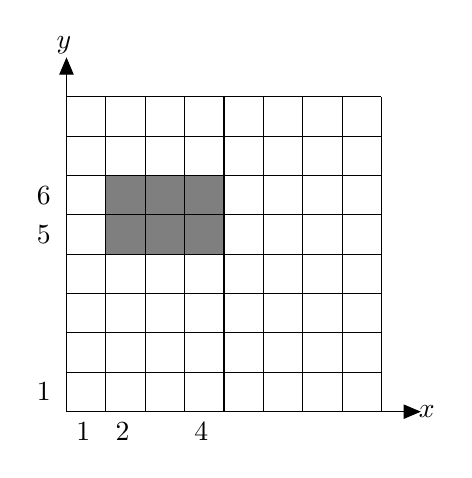
\begin{tikzpicture}[scale=.5]
\begin{scope}
    \draw (1, 1) grid (9, 9);
	\fill[black,fill opacity=0.5] (2,5) rectangle (5,7);
	\draw[triangle 45-triangle 45] (1,10) -- (1,1) -- (10,1);
\tikzset{anchor=west}
\node at (2,0.5) {$2$};
\node at (4,0.5) {$4$};
\node at (1,0.5) {$1$};
\node at (0,1.5) {$1$};
  \node at (0,6.5) {$6$};
  \node at (0,5.5) {$5$};
 \node at (0.5,10.3) {$y$};
  \node at (9.7,1) {$x$};
  %  \draw[very thick, scale=3] (0, 0) grid (3, 3);
\end{scope}
\end{tikzpicture}
\caption{$x= [2,4], y=[5,6]$}
\label{fig:mrqed-alice}
\end{subfigure}%
\begin{subfigure}[t]{.33\textwidth}
\centering
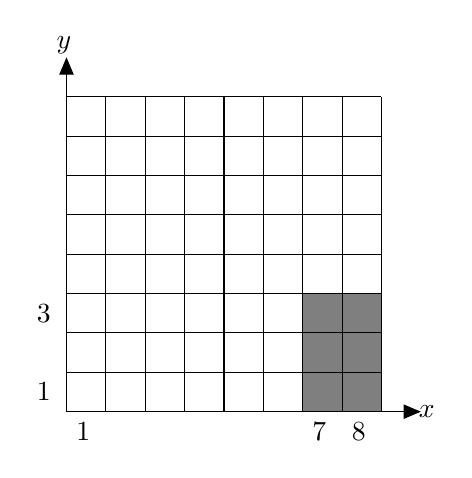
\begin{tikzpicture}[scale=.5]
\begin{scope}
    \draw (1, 1) grid (9, 9);
    \draw[triangle 45-triangle 45] (1,10) -- (1,1) -- (10,1);
	\fill[black,fill opacity=0.5] (7,1) rectangle (9,4);
\tikzset{anchor=west}
\node at (1,0.5) {$1$};
\node at (0,1.5) {$1$};
\node at (7,0.5) {$7$};
\node at (8,0.5) {$8$};
  \node at (0,3.5) {$3$};
    \node at (0.5,10.3) {$y$};
  \node at (9.7,1) {$x$};
  %  \draw[very thick, scale=3] (0, 0) grid (3, 3);
\end{scope}
\end{tikzpicture}
\caption{$x= [7,8], y=[1,3]$}
\label{fig:mrqed-bob}
\end{subfigure}%
\begin{subfigure}[t]{.33\textwidth}
\centering
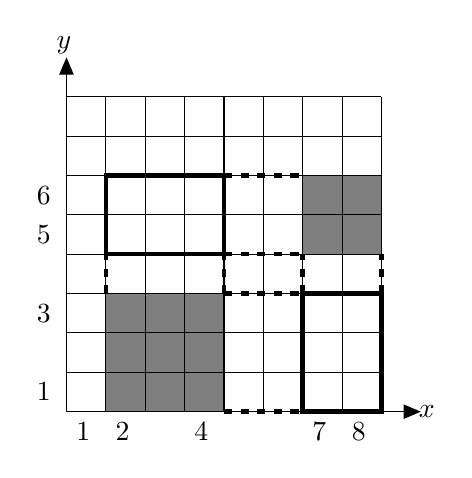
\begin{tikzpicture}[scale=.5]
\begin{scope}
    \draw (1, 1) grid (9, 9);
\draw[triangle 45-triangle 45] (1,10) -- (1,1) -- (10,1);
\draw[dashed, ultra thick] (2,4) -- (2,5);
\draw[dashed, ultra thick] (5,4) -- (5,5);
\draw[dashed, ultra thick] (5,4) -- (7,4);
\draw[dashed, ultra thick] (5,5) -- (7,5);
\draw[dashed, ultra thick] (5,7) -- (7,7);
\draw[dashed, ultra thick] (7,4) -- (7,5);
\draw[dashed, ultra thick] (9,4) -- (9,5);
\draw[dashed, ultra thick] (5,1) -- (7,1);

\draw[ultra thick] (7,1) rectangle (9,4);
\draw[ultra thick] (2,5) rectangle (5,7);



\fill[black,fill opacity=0.5] (2,1) rectangle (5,4);
\fill[black,fill opacity=0.5] (7,5) rectangle (9,7);
\tikzset{anchor=west}


\node at (1,0.5) {$1$};
\node at (0,1.5) {$1$};
\node at (7,0.5) {$7$};
\node at (8,0.5) {$8$};
  \node at (0,3.5) {$3$};

\node at (2,0.5) {$2$};
\node at (4,0.5) {$4$};
  \node at (0,6.5) {$6$};
  \node at (0,5.5) {$5$};
 \node at (0.5,10.3) {$y$};
\node at (9.7,1) {$x$};
  %  \draw[very thick, scale=3] (0, 0) grid (3, 3);
\end{scope}
\end{tikzpicture}
\caption{$x=[2,4], y= [1,3]$ and $x=[7,8], y= [6,5]$ after collusion}
\label{fig:mrqed-collude}
\end{subfigure}
\caption{Collusion  Problem}
\label{fig:collusion}
\end{figure}

However, this naive construction introduces the problem of collusion between different parties. Suppose Charlie obtains keys for the region $ x2=[7,8], y2=[1,3]$, shown in \cref{fig:mrqed-bob}. Bob is able to collude with Charlie to obtain the following additional keys for the regions $\{x1, y2\}$ and $\{x2, y1\}$, as shown in \cref{fig:mrqed-collude}.

Alternatively, we could trivially take the cross product of the different paths to the roots of each dimension. However, this results in a huge expansion in key size and ciphertext size since we now have  $\displaystyle \prod^{D} O(\log(n)) = O(\log(n))^D$ ciphertext size per frame, where $D$ is the number of dimensions. 

MRQED \cite{shi2007multi} presents a method that prevents the collusion attack without incurring an increase in key and ciphertext size. Instead of issuing $\{k_{x},k_{y}\}$, 
random variables are added to the key, producing $\{{u}_{x} k_{x}, u_{y} K_{y}\}$ , such that $u_{x} {u}_{y} = i$, where $i$ is an invariant to keep the scheme consistent. Using the same example, Alice would have $\{ \tilde{u}_{x} k_{x1}, \tilde{u}_{y} k_{y1} \}$ and Bob will have 
$\{ \tilde{u}_{x}'k_{x2}, \tilde{u}_{y}'k_{y2} \}$. Since $\tilde{u}_{x}\tilde{u}_{y}' \neq i$ and  $\tilde{u}_{x}'\tilde{u}_{y} \neq i$, Bob and Charlie are unable to collude with each other to obtain additional key information.

\subsection{Evaluation}
Both MRQED and ABE have similar space requirements, making heavy usage of tree structures. Moreover, MRQED scheme requires reorganization of data into a rigid predefined structure and is better employed for multi-dimensional data. On the other hand, ABE does not have such a limitation, as we are able to associate arbitrary names and values to the keys and ciphertexts, providing much more flexibility than MRQED.
% describe a few algorithms needed to  do ABE. 

\section{Key-Aggregate Cryptosystem}
\label{chap:kac}
Key-aggregate cryptosystem, or KAC \cite{chu2013key} is a scheme that allows use of a constant-size decryption key to decrypt any subset of ciphertexts. 

In this scheme, messages are encrypted under predefined ciphertext classes, and are identified by an index. To share keys belonging to ciphertext classes $1,3,6$, Alice will have to send $\{k_1, k_3, k_6\}$ to Bob, which is not efficient.

KAC provides a mechanism to aggregate the keys into a single key called an aggregate key ($K_S$) which is constant-size. For this example, Alice aggregates $k_1, k_3, k_6$ into a constant-size aggregate key $K_S$, where $S=\{1,3,6\}$. She then forwards $K_S$ along with a public parameter (\texttt{param}) to Bob. Bob is able use $K_S$ together with \texttt{param} to decrypt ciphertext classes belonging to either $1$, $3$ or $6$. $K_S$ is constructed to be collusion-resistant. 

\subsection{Realization of KAC}

KAC provides the power to decrypt messages belong to a set of ciphertext classes using only a constant-size key. The 5 algorithms of KAC is shown in \cref{tab:kac-algo}. We will not go into the details of the construction of KAC in this section.

%\begin{description}
%\item[Setup] \hfill \\
%Input: Security parameter ($1^{\lambda}$), Number of ciphertext classes ($n$) \\
%Output: Public parameter ($\texttt{param} = \langle g, g_1, \dots , g_n,g{_n+2}, \dots, g_{2n} \rangle$)
%
%\item[KeyGen] \hfill \\
%Input: \texttt{param} \\
%Output: Public key ($\texttt{pk} = v$),  Master secret key ($\texttt{msk} = \gamma$)
%
%\item[Encrypt] \hfill \\
%Input: \texttt{pk}, index $1 \leq i \leq n$ denoting ciphertext class, massage (\texttt{msg}), \texttt{param} \\
%Output: ciphertext ($\mathfrak{C}$)
%
%\item[Extract] \hfill \\
%Input: \texttt{msk}, set of ciphertext classes ($S$), \texttt{param} \\
%Output: Aggregate key ($\displaystyle  K_s = \prod_{j \in S} g^{\gamma}_{n+1-j}$)
%
%\item[Decrypt] \hfill \\
%Input: $K_s, S, i,$ $\mathfrak{C}$, \texttt{param} \\
%Output: \texttt{msg} if $i \in S$
%
%\end{description}


\begin{table}[h]
\begin{tabular}{|l|p{0.44\textwidth}|p{0.36\textwidth}|}
\hline
\textbf{Algorithm} & \textbf{Inputs}                                                                                        & \textbf{Outputs}                                                                                 \\ \hline
\textbf{Setup}              & Security parameter ($1^{\lambda}$), number of ciphertext classes ($n$)                                 & Public parameter ($\texttt{param} = \langle g, g_1, \dots , g_n,g_{n+2}, \dots, g_{2n} \rangle$) \\ \hline
\textbf{KeyGen}             & \texttt{param}                                                                                         & Public key ($\texttt{pk} = v = g^\gamma$), Master secret key ($\texttt{msk} = \gamma$)                                                           \\ \hline
\textbf{Encrypt}            & \texttt{pk}, index $1 \leq i \leq n$ denoting ciphertext class, massage (\texttt{msg}), \texttt{param} & ciphertext ($\mathfrak{C} = \langle c_1, c_2, c_3 \rangle$)                                                                         \\ \hline
\textbf{Extract}            & \texttt{msk}, set of ciphertext classes ($S$), \texttt{param}                                          & Aggregate key ($\displaystyle  K_S = \prod_{j \in S} g^{\gamma}_{n+1-j}$)                        \\ \hline
\textbf{Decrypt}            & $K_S, S, i,$ $\mathfrak{C}$, \texttt{param}                                                               & \texttt{msg} if $i \in S$                                                                        \\ \hline
\end{tabular}

\caption{KAC algorithms}
\label{tab:kac-algo}
\end{table}


%The \textbf{KeyGen} stage in KBE is analogous to the \textbf{Setup} stage in ABE. The counterpart of \textbf{Extract} stage in ABE would be \textbf{KeyGen}. 
Alice uses \texttt{pk} generated in \textbf{KeyGen} stage along with ciphertext class $i$ to encrypt \texttt{msg}, producing $\mathfrak{C}$. Bob with access rights to set $S$ of ciphertext classes is entrusted with $K_S$.  $K_S$ can be used to decrypt $\mathfrak{C}$ if $i \in S$.  It is theoretically impossible for decryption keys to be constant in size for all possible combinations of ciphertext classes. The constant-size aggregate key is archived by encapsulating and delegating the information needed for encryption and decryption to \texttt{param}, which is $\Theta(n)$ in size.

Although the use of $K_S$ together with \texttt{param} is not of $O(1)$ in size. However, such a scheme can be very beneficial in the context of unsecured cloud storage. For instance, Alice stores $\mathfrak{C}$ and \texttt{param} in the cloud and sends $K_S$ to Bob via a private channel. In this case, the small size of $K_S$ in this case is desirable because the private channel may be limited in bandwidth. Thus, it can be seen that KAC is an excellent scheme for handling time-series data, as data points can be represented as distinct ciphertext classes.

\subsection{Key Extension}

Since the number of ciphertext classes $n$ has to be be defined during \textbf{Setup}, extending the ciphertext classes using existing \texttt{msk} and \texttt{pk} can be difficult. In~\cite{chu2013key}, an extension scheme is proposed with $l$ ($v, \gamma$) key pairs, supporting up to $O(ln)$ ciphertext classes. Each class is now represented by a 2-dimensional coordinate $\{ (i, j) | 1 \leq i \leq l, 1 \leq j \leq n\}$, where $\texttt{pk}_l = \{ v_1,\dots v_l \}, \texttt{msk} = \{\gamma_1, \dots \gamma_l\}$ under the new scheme.

\begin{figure}[h]
\centering
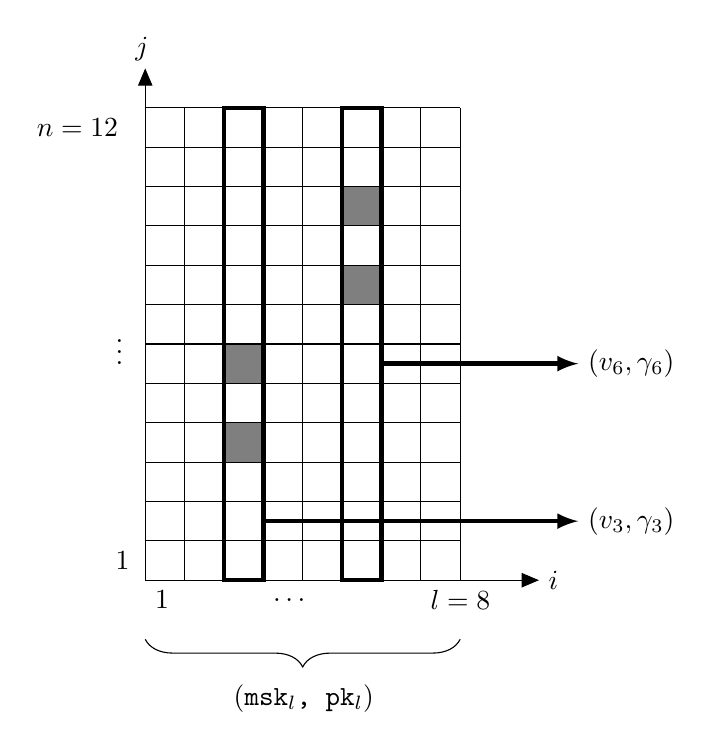
\begin{tikzpicture}[scale=.5]
\begin{scope}
    \draw (1, 1) grid (9,13);
    \draw[triangle 45-triangle 45] (1,14) -- (1,1) -- (11,1);
    %\draw[-latex, thick] (3.5,4.5) -- (15,4.5);
    \draw[ultra thick, -latex] (4,2.5) -- (12, 2.5);
 \draw[ultra thick, -latex] (7,6.5) -- (12, 6.5);

 \fill[black, fill opacity=0.5] (6,10) rectangle (7,11);
 \fill[black, fill opacity=0.5] (6,8) rectangle (7,9);

 \fill[black, fill opacity=0.5] (3,6) rectangle (4,7);
 \fill[black, fill opacity=0.5] (3,4) rectangle (4,5);

  \draw[ultra thick] (6,1) rectangle (7,13);
\draw[ultra thick] (3,1) rectangle (4,13);

\tikzset{anchor=west}
\node at (0.5,14.5) {$j$};

\node at (11,1) {$i$};
\node at (5.5,8.5) {};
\node at (1,0.5) {1};
%\node at (-2,1.5) {($v_1, \gamma_1$)};
\node at (4,0.5) {\dots};
\node at (8,0.5) {$l=8$};
\node at (0,7) {\vdots};
\node at (12,6.5) {$ (v_6, \gamma_6)$};
\node at (12,2.5) {$ (v_3, \gamma_3)$};
%\node at (-2,5.5) {($v_l, \gamma_l$)};
  %\node at (-4, 5.5)  {(\texttt{msk$_l$, pk$_l$})};
\node at (-2, 12.5)  {$n=12$};
\node at (0, 1.5)  {1};
  %  \draw[very thick, scale=3] (0, 0) grid (3, 3);
\draw [decorate,decoration={brace,amplitude=10pt,mirror}] (1,-0.5) -- (9,-0.5) ;
\node at (3,-2) {(\texttt{msk$_l$, pk$_l$})};
% node [black,midway,yshift=-1cm] {(\texttt{msk$_l$, pk$_l$})};
\end{scope}
\end{tikzpicture}
\caption{KAC key extension} \label{fig:kac-extend}
\end{figure}

%To release $K_s$ for the points $(3,4), (3,6), (6,8)$, Alice simply has to release. 
As shown in \cref{fig:kac-extend}, points lying on the same ``column'' ($i$ value) are encrypted with the same keys and can be aggregated. Column 3 is associated with {$ (v_3, \gamma_3)$} while column 6 is associated with {$ (v_6, \gamma_6)$}. Data points in different columns are encrypted with different keys and cannot be aggregated. Overall, the number of keys that Alice has to send to Bob is dependent on the number of ``columns'' which data points span. 

The points $(3,4), (3,6), (6,8), (6,10)$ spans 2 columns, column 3 and 6. Hence 2 keys are released, $K_S = \{ \displaystyle  \prod_{(3,j), j \in \{4,6\} } g^{\gamma_3}_{n+1-j},  \prod_{ (6,j), j \in  (8,10)} g^{\gamma_6}_{n+1-j}$ \}. Notice that a single aggregate key $\displaystyle \prod_{(3,j), j \in \{4,6\} } g^{\gamma_3}_{n+1-j}$ is enough to decrypt both (3,4) and (3,6) because those two points have the same $i$ value, lying in the same column. Likewise, a single aggregate key $\displaystyle \prod_{ (6,j), j \in  (8,10)} g^{\gamma_6}_{n+1-j}$ is sufficient to decrypt $(6,8), (6,10)$.

\subsection{Evaluation}
KAC presents a viable scheme that can potentially reduce decryption key size since the aggregate key is constant in size. However, the linear-size \texttt{param} is a large storage overhead that has to be taken into consideration. The decryption process may also not be sufficiently efficient for large quantities of plaintext.

%it could be hard to represent data with more than 2 dimensions with KAC as there is no inherent hierarchy structure in KAC. It was suggested in \cite{chu2013key} that ciphertext class for different purposes should be encrypted under different {$ (v, \gamma)$}. 





\chapter{Security Model}
\label{chap:model}
In this chapter, we will discuss our model proposed for secure storage outsourcing. We will also consider the runtime and security requirements of the system. 

\section{Entities}
\label{sec:scheme}
We first consider the entities involved in our proposed model.   %\cite{kamara2010cryptographic} has highlighted the security properties that a virtual private storage service must provide, mainly in aspects of confidentiality, integrity and non-repudiation.  The security model is constructed based on these 3 properties. 
There are $4$ entities involved.

\paragraph{Public Cloud (RC)} A outsourced service provider hosting the encrypted files. It is assumed that RC has ample storage and bandwidth. In our model, RC merely provides storage services and has low computational capabilities.
\paragraph{Key Granter (KG)} A trusted server responsible for key management, key distribution, user authentication and access mediation. In actual implementations, this is likely to be an internal server hosted by the organization. In our model, user authentication and access control is assumed to be handled by an external verifier which is not in the scope of our project.

\paragraph{Data Owner (DO)} The author of the file containing time-series data. DO is responsible for key generation and file encryption. The keys generated will be uploaded to KG while the encrypted file will be uploaded to RC.
\paragraph{Authorized User (AU)} A user of the system who is authorized to decrypt an encrypted file hosted in RC. Depending on access rights, AU may only be able to decrypt specific regions of the file.


\section{Interactions}
\label{sec:interact}
The entities operate with one another to perform tasks. These tasks can be classified into four main phases. The phases are \textbf{Synthesis}, \textbf{Upload}, \textbf{Retrieval} and \textbf{Key Distribution}. \cref{fig:sec-model} illustrates the order of interactions between the various entities. We classify the interactions into 4 different phases.

\begin{figure}[H]
\centering
\tikzstyle{txtbox}=[rectangle, minimum width=50pt,minimum height=30pt,draw=black]
\tikzstyle{txtbox-circle}=[circle, minimum width=50pt, draw=black]
\tikzstyle{trap}=[circle, minimum width=70pt,minimum height=40pt,draw=black]
\begin{tikzpicture}

\definecolor{light-gray}{gray}{0.95}
\node [txtbox] (do) {DO} ;
\node [txtbox-circle, below of=do, node distance=95pt] (kg) {KG} ;
\node [txtbox, right of=do, node distance=170pt] (rc) {RC} ;
\node [txtbox, right of=kg, node distance=170pt] (au) {AU} ;

\path[-latex,every node/.style={draw, circle}]

%(do) edge[bend right] node[left]{1} (kg)
(do) edge[loop left] node[left]{1} (do)
(do) edge node[left]{2} (kg)



(do) edge node[above]{3} (rc)
(rc) edge node[right] {4} (au)
(au) edge[bend right] node[above] {5} (kg)
(kg) edge[loop left] node[left]{6} (kg)
(kg) edge[bend right] node[above] {7} (au)
(au) edge[loop right] node[right]{8} (au);

\end{tikzpicture}
\caption{Interactions between entities} \label{fig:sec-model}
\end{figure}

\paragraph{Synthesis} 
\begin{enumerate}[noitemsep,nolistsep]

\item DO generates a set of master keys. Using the master keys, DO derives a set of symmetric frame keys and uses the frame keys to encrypt the video frames. 
\end{enumerate}

\paragraph{Upload}
\begin{enumerate}[resume,noitemsep,nolistsep]
\item DO forwards the master keys as well as other essential parameters to KG.

\item DO uploads the encrypted video along with other public parameters/data to RC. 
\end{enumerate}

\paragraph{Retrieval}
\begin{enumerate}[resume,noitemsep,nolistsep]
\item AU downloads the encrypted video and public data from RC.

\item AU requests for a meta-key from KG to decrypt specific video frames in set $S$. 
\end{enumerate}

\paragraph{Key Distribution}
\begin{enumerate}[resume,noitemsep,nolistsep]
\item KG uses an external verifier to verify the identity as well as the access rights of AU. If AU indeed has rights to $S$, KG computes the meta-key for frames in $S$ using the master key.

\item KG forwards meta-key to AU.

\item Using the meta-key from KG as well as public data from DO, AU is able to derive keys for video frames in $S$. 

\end{enumerate}



This model can be realized using encryption schemes such as KP-ABE, MRQED or KAC. DO uses these schemes to encrypt the frame keys, which are symmetric keys such as DES or AES. Next, the encrypted frame keys are uploaded along with the encrypted video. AU downloads the encrypted video frames along with the encrypted frame keys. The meta-key serves as a decryption key to the encrypted frame keys. Using the meta-key, AU can decrypt the encrypted frame keys, allowing for video decryption. 


\section{Performance Requirements}

\paragraph{KG Bandwidth} Since KG is hosted internally within the organization, bandwidth is at a premium. Therefore, the information transferred to/from KG should be kept to the minimal. As key transfers between KG to AU during \textbf{Key Distribution} are likely to occur frequently, the meta-key size should be of size $O(1)$. In \textbf{Upload} phase, keys are transferred from DO to KG and the bandwidth costs incurred should ideally be $O(\log(n))$.  


\paragraph{KG Storage} Maintaining a huge storage archive within the organization is costly. A huge data store also means that data is likely to be distributed over a few servers, increasing the chances of possible key leakage. Hence, the amount of key information stored for a single video is capped at $O(\log(n))$.

\paragraph{RC Bandwidth/Storage} In \textbf{Upload}, DO sends the encrypted video frames and other relevant public data to RC. AU then downloads these data in \textbf{Retrieval} phase. Since RC is an outsourced storage provider, it is assumed that bandwidth and storage costs are cheap. Even so, the storage and bandwidth should be of the same order of magnitude as the size of the video (number of frames). Hence, both storage and bandwidth costs are capped at $O(n)$.

\paragraph{Encryption/Decryption Time} Video encryption and decryption should be faster than the video's frame rate to meet real-time requirements. For purposes of this project, the frame rate of all video data is set to be 24 FPS. This also means that asymptotic runtimes of encryption and decryption are capped at $O(n)$.




\section{Security Requirements}
In this scheme, the only trusted entity is KG. The system should be secure against the following attacks.


\paragraph{Unauthorized data access}The goal of the adversarial AU is to obtain frame keys that is not within his/her access rights.  We do not consider attacks which are targeted at the external verifier (e.g. impersonating as another AU with more access rights).
%The adversary AU has access rights to a set of video frame keys $(S)$ who is capable of requesting KG for decryption keys in S. The adversary's goal is to be able to obtain key $k$ such that  $v \not\in S$. 

\paragraph{Malicious/Spoofed RC} The adversary is either a malicious RC or an entity spoofing as a trusted RC. He is able to communicate with the DO and AU and convince them that he is a trusted RC. His goal is to be able to extract plaintext information apart from metadata which is derivable from ciphertext (size of video, frame count). 

\paragraph{KG Spoofing} The adversary is able to communicate with DO and AU. His goal is to convince DO and AU that he is a trusted KG. By doing so, he is able to issue his own encryption/decryption keys, allowing him to gain access to the plaintext.

\paragraph{Collusion-resistant} Bob and Charlie are AU with access rights to the set of keys $S_{B}$ and $S_{C}$ respectively. Bob and Charlie should not be able obtain key $k$ where $k \not\in S_{B} \cup S_{C}$.




\chapter{Preliminary Analysis}
\label{chap:prelim}
For this project, we have looked into the use of KAC~\cite{chu2013key} and KP-ABE~\cite{lewko2010revocation} as possible basis of implementations for our scheme. In this chapter, we present some in-depth performance analysis and comparisons between these two schemes.

All empirical data are gathered from prototypes built using Charm~\cite{charm13} cryptographic framework, running on Macbook Air 2013 (Intel Core-i7-4650u). Symmetric pairings over Type-A (supersingular) curves  with a base field of $512$ bits are chosen as the underlying pairing group. No pre-computation tables were used for group exponentiation.

\section{Space Requirements}



\subsection{Meta-Key}
\label{sec:meta-key-store}

The meta-key or aggregate key is an important part of our system. The meta-key allows the user to decrypt the symmetric frame keys stored in RC, which can then be used to decrypt the video frames.
 
In KP-ABE, using the ``bag of bits'' notation introduced in \cref{sec:abe-range}, it is possible to construct a meta-key that is  logarithmic in size for a contiguous range\footnote{Sequence in the form of $\{i,i+1,i+2, \dots\}$} of frames. Hence, $MK$ generated by the KP-ABE's \textbf{KeyGen} algorithm can be constructed with just $O(log(n))$ group elements. In KAC, the aggregate key $(K_S)$ generated by the \textbf{Extract} algorithm serves as the meta-key. $K_S$ is constant in size, comprising of a single group element. 

\cref{fig:kac-abe-aggregate-size} compares differences in key size with varying video size for decryption of a single contiguous range. For KP-ABE, the key size displays a logarithmic growth rate with respect to $n$ while KAC generates constant-size keys for all values of $n$. 

For meta-keys that are non-contiguous,  KP-ABE may produce keys of $O(|S|)$ in size because of the need to encode individual values as separate attributes, with $S$ representing the set of frames that the meta-key is authorized to decrypt. The ``bag of bits'' notation can only be used for represent contiguous ranges.  KAC on the other hand is able to consistently produce keys of size $O(1)$ even for non-contiguous values. For simplicity of analysis, we shall be comparing storage and runtime performance that is of contiguous in nature in the subsequent sections.

\begin{figure}[H]
\centering
\begin{minipage}[t]{0.5\textwidth}
\begin{tikzpicture}

\begin{loglogaxis}[xlabel={$n$},width=1\linewidth,ylabel={bytes},title={Contiguous $S$}]%, legend style={at={(1,0.5)},anchor=east}, cycle list name=black white]


% Graph column 2 versus column 0
\addplot+[smooth] table[x index=0,y index=1,col sep=comma] {../Code/SS512/abe_aggregate_size.csv};
\addplot+[mark=triangle, smooth] table[x index=0,y index=1,col sep=comma] {../Code/SS512/kac_aggregate_size.csv};
%\addplot+[mark=x, smooth]  table[x index=0,y index=1,col sep=comma] {../Code/SS1024/kac_aggregate_size.csv};
\addlegendentry{KP-ABE}
\addlegendentry{KAC}% y index+1 since humans count from 1
%\addlegendentry{KAC (SS1024)}% y index+1 since humans count from 1


\end{loglogaxis}
\end{tikzpicture}

\caption{Meta-key size}
\label{fig:kac-abe-aggregate-size}
\end{minipage}~
\begin{minipage}[t]{0.5\textwidth}
\centering
\begin{tikzpicture}

\begin{loglogaxis}[xlabel={$n$},width=1\linewidth,ylabel={bytes}, legend pos=north west]


% Graph column 2 versus column 0
%\addplot+[smooth] table[x index=0,y index=1,col sep=comma] {../Code/SS1024/kac_private_space.csv};
\addplot+[smooth] table[x index=0,y index=1,col sep=comma] {../Code/SS512/kac_private_space.csv};
\addplot+[mark=x, smooth] table[x index=0,y index=1,col sep=comma] {../Code/SS512/abe_private_space.csv};
\addlegendentry{KAC}% y index+1 since humans count from 1
\addlegendentry{KP-ABE}% y index+1 since humans count from 1

% Graph column 1 versus column 0    
%\addplot table[x index=0,y index=1,col sep=comma] {datax.dat};
%\addlegendentry{Column 2}

\end{loglogaxis}
\end{tikzpicture}
\caption{KG Storage}
\label{fig:kg-storage}
\end{minipage}

\end{figure}


\subsection{KG -- Private Storage}
\label{sec:kac-private}
The KG has to contain a minimal amount of parameters for key computation and these parameters have to be stored in KG. 


\begin{table}[H]
    \begin{tabular}{|l|l|l|l|}
    \hline
    ~      & Master Key      & Public Key & Public Parameters      \\ \hline
    KAC    & $1$ prime element &  $1$ group element & $2n$ group elements \\ \hline
    KP-ABE & $3$ prime elements & $5$ group elements & --                  \\ \hline
    \end{tabular}

    \caption{KG storage requirements}
        \label{tab:kg-storage}
\end{table}


KP-ABE's \textbf{Key Generation} algorithm requires the only master key and public key as inputs, and these $2$ inputs are constant in size. KAC's \textbf{Extract} algorithm, which is analogous to KP-ABE's \textbf{Key Generation}, requires the master key and a linear-size public parameter \texttt{param}. As summarized in \cref{tab:kg-storage}, because of the need to store a linear-size parameter required for the generation of the meta-key, the amount of storage required by KAC is much more than KP-ABE. In \cref{fig:kg-storage}, we see that KG storage required by KG increases to more than $2^{20}$ for $n>2^{12}$. In this aspect, KP-ABE is a better choice as opposed to KAC.


\subsection{RC -- Public Storage}
\label{sec:kac-public}

\begin{table}[H]
    \begin{tabular}{|l|l|l|l|}
    \hline
    ~      & Public Key        & Ciphertext (per Frame)                       & Public Parameters     \\ \hline
    KAC    & $1$ group element  & $3$ group elements                         & $2n$ group elements \\ \hline
    KP-ABE & $5$ group elements & $O(\log(n))$ attributes and group elements & --                  \\ \hline
    \end{tabular}
        \caption{RC storage requirements}
    \label{tab:rc-storage}
\end{table}


\begin{figure}
\centering
\begin{subfigure}[t]{0.5\textwidth}

\begin{tikzpicture}

\begin{axis}[xlabel={$n$},,ylabel={bytes}, log basis y=2]

% Graph column 2 versus column 0
\addplot+[smooth, mark=square] table[x index=0,y index=1,col sep=comma] {../Code/SS512/abe_public_space.csv};
\addplot+[smooth] table[x index=0,y index=1,col sep=comma] {../Code/SS512/kac_public_space.csv};

\addlegendentry{KP-ABE}
\addlegendentry{KAC}% y index+1 since humans count from 1

%\addlegendentry{72FPS}
% Graph column 1 versus column 0    
%\addplot table[x index=0,y index=1,col sep=comma] {datax.dat};
%\addlegendentry{Column 2}

\end{axis}
\end{tikzpicture}

\caption{Linear Scale}
\label{fig:rc-storage-linear}
\end{subfigure}~
\begin{subfigure}[t]{0.5\textwidth}

\begin{tikzpicture}

\begin{loglogaxis}[xlabel={$n$},,ylabel={bytes}, log basis y=2]

% Graph column 2 versus column 0
\addplot+[smooth, mark=square] table[x index=0,y index=1,col sep=comma] {../Code/SS512/abe_public_space.csv};
\addplot+[smooth] table[x index=0,y index=1,col sep=comma] {../Code/SS512/kac_public_space.csv};
%\addplot+[no markers, domain=1:32768]{x/72};
\addlegendentry{KP-ABE}
\addlegendentry{KAC}
%\addlegendentry{72FPS}
% Graph column 1 versus column 0    
%\addplot table[x index=0,y index=1,col sep=comma] {datax.dat};
%\addlegendentry{Column 2}

\end{loglogaxis}
\end{tikzpicture}
\caption{Log-Log scale}

\end{subfigure}
\caption{RC storage}
\label{fig:rc-storage}
\end{figure}

RC is where we store the encrypted video, as well as the encrypted symmetric keys for the video frames. As summarized in \cref{tab:rc-storage}, the use ``bag of bits'' notation results in logarithmic-size ciphertext. Hence, KP-ABE produces ciphertext that is $O(\log(n))$ in $O(n\log(n))$ storage for $n$ frames. Ciphertext generated by KAC is constant size, resulting in $O(n)$ storage for $n$ frames. \cref{fig:rc-storage} shows the deviation in storage for KP-ABE and KAC for increasing $n$. The difference in storage is obvious when plotted against a linear scale, as shown in \cref{fig:rc-storage-linear}.




\section{Runtime}



\subsection{Setup}

\begin{table}[H]
    \begin{tabular}{|l|l|l|l|l|l|}
    \hline
    ~      & Pairing & Exponentiation        & Multiplication & Division & Hash \\ \hline
    KAC    & $1$  & $2(2n-1) + 1 = \Theta(n)$ & 0              & 0        & 0    \\ \hline
    KP-ABE & $O(1)$  & $O(1)$                & $O(1)$         & 0        & 0    \\ \hline
    \end{tabular}
    \caption{Running complexity for the setting up of parameters}
	\label{tab:kac-abe-setup}
\end{table}

Both KAC and KP-ABE schemes have a setup phase to generate the parameters required for encryption/decryption. As shown in \cref{tab:kac-abe-setup}, the \textbf{Setup} phase of KP-ABE takes only constant time, generating private and public keys of size $O(1)$. The \textbf{Setup} phase in this case will be performed by DO. DO encrypts the symmetric keys of the video using KP-ABE. Since only the public key is transferred from DO to KG, the bandwidth required is $O(1)$.

For KAC, the setup process consists of \textbf{Setup} and \textbf{KeyGen} algorithms. The \textbf{Setup} phase is where the computation of \texttt{param} takes place while KAC's \textbf{KeyGen} algorithm is analogous to the \textbf{Setup} algorithm of KP-ABE where the generation of public and private keys take place. Since DO is required to transfer \texttt{param} to KG, $\Theta(n)$ bandwidth is required. Also, due to the need to generate $2n$ group elements, KAC incurs a larger runtime complexity than KP-ABE.

Instead of transferring $\Theta(n)$ size \texttt{param} to KG, DO could transfer a constant-size $\alpha$ to KG, where $\alpha$ is a secret exponent used in KAC's \textbf{Setup} algorithm to generate \texttt{param}. KG then generates $2n$ group elements from $\alpha$. However, this method limits the number of DOs KG can support since generating \texttt{param} is computationally expensive. 

\subsection{Encryption}
\begin{table}[H]
    \begin{tabular}{|l|l|l| l | l | l |}
    \hline
    ~      & Pairing & Exponentiation & Multiplication & Division & Hash         \\ \hline
    KAC    & $1$     & $3$            & $2$            & $0$      & $0$          \\ \hline
    KP-ABE & $0$     & $O(log(n))$   & $O(1)$         & $0$      & $O(log(n))$ \\ \hline
    \end{tabular}
    \caption{Encryption complexity per frame}
    \label{tab:kac-abe-encryption}
\end{table}
\Cref{tab:kac-abe-encryption} summarizes the number of operations it takes for both setup and encryption. We see that KP-ABE has a runtime complexity of $O(\log(n))$ to encrypt a single piece of ciphertext. This translates to $O(n\log(n))$ for $n$ frames. KAC on the other hand, takes constant time to encrypt each piece of plaintext, resulting in a total complexity of $\Theta(n)$ for $n$ frames. In \cref{fig:kac-abe-setup} and \cref{fig:kac-abe-setup-loglog} which shows the time it takes for both setup and encryption, we see that there is a divergence in the runtime for large $n$ values, especially in \cref{fig:kac-abe-setup} where a linear scale is used. In fact, we see that KAC is efficient enough to be able to encrypt keys for a 24FPS video in real-time.



\begin{figure}[H]
\centering
\begin{subfigure}{0.5\textwidth}

\begin{tikzpicture}

\begin{axis}[xlabel={$n$},,ylabel={Time (s)}, log basis y=2]

% Graph column 2 versus column 0
\addplot+[smooth, mark=square] table[x index=0,y index=1,col sep=comma] {../Code/SS512/abe_encrypt_time.csv};
\addplot+[smooth] table[x index=0,y index=1,col sep=comma] {../Code/SS512/kac_encrypt_time.csv};
\addplot+[no markers, domain=1:32768, dashed]{x/24};
%\addplot+[no markers, domain=1:32768, dotted, thick, black]{x/72};
\addlegendentry{KP-ABE}
\addlegendentry{KAC}% y index+1 since humans count from 1
\addlegendentry{24FPS}% y index+1 since humans count from 1
%\addlegendentry{72FPS}
% Graph column 1 versus column 0    
%\addplot table[x index=0,y index=1,col sep=comma] {datax.dat};
%\addlegendentry{Column 2}

\end{axis}
\end{tikzpicture}
\caption{Linear Scale}
\label{fig:kac-abe-setup}
\end{subfigure}~
\begin{subfigure}{0.5\textwidth}

\begin{tikzpicture}

\begin{loglogaxis}[xlabel={$n$},,ylabel={Time (s)}, log basis y=2]

% Graph column 2 versus column 0
\addplot+[smooth, mark=square] table[x index=0,y index=1,col sep=comma] {../Code/SS512/abe_encrypt_time.csv};
\addplot+[smooth] table[x index=0,y index=1,col sep=comma] {../Code/SS512/kac_encrypt_time.csv};
\addplot+[no markers, domain=1:32768, dashed]{x/24};
%\addplot+[no markers, domain=1:32768]{x/72};
\addlegendentry{KP-ABE}
\addlegendentry{KAC}% y index+1 since humans count from 1
\addlegendentry{24FPS}% y index+1 since humans count from 1
%\addlegendentry{72FPS}
% Graph column 1 versus column 0    
%\addplot table[x index=0,y index=1,col sep=comma] {datax.dat};
%\addlegendentry{Column 2}

\end{loglogaxis}
\end{tikzpicture}
\caption{Log-Log scale}
\label{fig:kac-abe-setup-loglog}
\end{subfigure}
\caption{Setup $+$ Encryption time}
\end{figure}



\subsection{Meta-key Generation}

%The time it takes for the KG to respond to AU's request is dependent on the time it takes for the KG to generate the meta keys. 
\begin{table}[H]
    \begin{tabular}{|l|l|l|l|l|l|}
    \hline
    ~      & Pairing & Exponentiation & Multiplication & Division & Hash         \\ \hline
      KAC & $0$     & $1$          & $|S|$         & $0$    & $0$            \\ \hline
    KP-ABE    & $0$     & $O(\log(n))$   & $O(\log(n))$   & $0$        & $O(\log(n))$ \\ \hline
  
    \end{tabular}
    \caption{Meta-key generation complexity (Contiguous Range)}
    \label{tab:kac-abe-extract}
\end{table}


The response time to AU's request depends on the time it takes for KG to generate the meta keys. In \cref{tab:kac-abe-extract}, we see that KAC's \textbf{Extract} algorithm is dependent on $S$ unlike KP-ABE's \textbf{KeyGen} algorithm. Since $|S|\leq n$, the runtime complexity of KAC may be as high as $O(n)$. In \cref{fig:kac-abe-extract}, we see that the actual runtime of KP-ABE is much slower than than KAC, despite KAC having a larger complexity. This is because KP-ABE requires $O(\log(n))$ exponentiations which are more computationally intensive than multiplications.


\begin{figure}[H]

\centering

\begin{minipage}[t]{.5\textwidth}
\begin{tikzpicture}
\selectcolormodel{gray}
\begin{loglogaxis}[xlabel={$|S|$},width=1\linewidth,ylabel={Time (s)},width=\textwidth, legend pos=south east, title={Contiguous $S$}]

% Graph column 2 versus column 0
\addplot+[smooth, mark=triangle] table[x index=0,y index=1,col sep=comma] {../Code/SS512/abe_extract_time.csv};

\addplot+[smooth] table[x index=0,y index=1,col sep=comma] {../Code/SS512/kac_extract_time_fast.csv};

\addlegendentry{KP-ABE}
\addlegendentry{KAC}


% Graph column 1 versus column 0    
%\addplot table[x index=0,y index=1,col sep=comma] {datax.dat};
%\addlegendentry{Column 2}

\end{loglogaxis}
\end{tikzpicture}
\caption{Meta-key generation time (contiguous range)}
\label{fig:kac-abe-extract}
\end{minipage}%
\begin{minipage}[t]{.5\textwidth}
\begin{tikzpicture}

\begin{loglogaxis}[width=0.8\textwidth, xlabel={$|Q|$},ylabel={Time (s)}, title={$n=65536, Q=S,$ contiguous $Q$}, width=\textwidth]

% Graph column 2 versus column 0
\addplot+[smooth, mark=triangle] table[x index=0,y index=1,col sep=comma] {../Code/SS512/kac_normal_decrypt_time.csv} ;

\addplot+[smooth, mark=x] table[x index=0,y index=1,col sep=comma] {../Code/SS512/abe_decrypt_time.csv};




\addplot+[no markers, domain=1:32768, dashed]{x/24};
%\addplot+[no markers, domain=1:32768, dotted, thick, black]{x/72};

\addlegendentry{KAC}
\addlegendentry{KP-ABE}



\addlegendentry{24 FPS}
%\addlegendentry{72 FPS}
% Graph column 1 versus column 0    
%\addplot table[x index=0,y index=1,col sep=comma] {datax.dat};
%\addlegendentry{Column 2}

\end{loglogaxis}
\end{tikzpicture}
\caption{Decryption Time}
\label{fig:kac-abe-decrypt}
\end{minipage}
\end{figure}


\subsection{Decryption}
\begin{table}[h]
    \begin{tabular}{|l|l|l|l|l|l|}
    \hline
    ~      & Pairing      & Exponentiation & Multiplication & Division     & Hash         \\ \hline
    KAC    & $2$          & $0$            & $2|S| + 1$     & $1$          & $0$          \\ \hline
    KP-ABE & $O(\log(n))$ & $O(\log(n))$   & $O(\log(n))$   & $O(\log(n))$ & $O(\log(n))$ \\ \hline
    \end{tabular}
    \caption{Decryption complexity per frame}
    \label{tab:kac-abe-decrypt}
\end{table}

AU may request for a meta-key that is able to decrypt keys in the set $S$. Instead of decrypting all of the frame keys in $S$, the AU may choose to decrypt just a subset of the keys. We denote this decryption set as $Q$, where $Q \subseteq S$. In \cref{tab:kac-abe-decrypt}, we see that decryption for KAC has a complexity of $\Theta(|S|)$ per ciphertext, or $|Q|\Theta|S| = O(|S^2|)$ for decryption of $|Q|$ frames. In comparison, KP-ABE requires $O(\log(n))$ per ciphertext, or $|Q|O(\log(n))$ for $|Q|$ frames.  Experimental results in \cref{fig:kac-abe-decrypt} show that the runtime of KAC begins to exceeds KP-ABE for $|Q| > 2^{12}$ when KAC's multiplications outpaces KP-ABE's operations.  For $|Q|>2^8$, we see that KP-ABE's decryption rate outpaces the frame rate of a 24FPS video.
\section{Conclusion}

\begin{table}[h]
\centering
\begin{subtable}{1\textwidth}
\centering
    \begin{tabular}{|l|l|l| p{0.4\textwidth}|}
    \hline
    ~      & KG     & RC            & Meta-key (KG $\to$ AU)                                    \\ \hline
    KAC    & $\Theta(n)$ & $\Theta(n)$        & $O(1)$                                                    \\ \hline
    KP-ABE & $O(1)$ & $O(n\log(n))$ & Contiguous: $O(\log(n))$ \newline Non-contiguous: $O(|S|)$ \\ \hline
    \end{tabular}
    \caption{Storage}
\end{subtable}
\begin{subtable}{1\textwidth}
\centering
    \begin{tabular}{|l|l|l|l|}
    \hline
    ~      & Setup $+$ Encryption                & Decryption       & Meta-key generation \\ \hline
    KAC    & $\Theta(n) + \Theta(n) = \Theta(n)$ & $|Q|\Theta(|S|)$ & $\Theta(|S|)$       \\ \hline
    KP-ABE & $1 + O(n\log(n)) = O(n\log(n))$     & $|Q|O(\log(n))$   & $O(\log(n))$         \\ \hline
    \end{tabular}
       \caption{Runtime}
     \end{subtable}
    \caption{Summary of storage and runtime requirements}
    \label{tab:summary}
\end{table}

Both KAC and KP-ABE have their strengths and weaknesses in both storage and runtime (\cref{tab:summary}). KAC has the advantage of producing meta-keys of size $O(1)$. KP-ABE on the other hand has a small storage footprint on KG, requiring only $O(1)$ storage. However, its construction based on access trees also means that it has disadvantages similar to GGM-tree. KP-ABE is also able to provide support for multi-dimensional data since key produced is collusion-resistant. Despite the slower decryption speed and large KG storage, we have chosen KAC as the implementation basis for our scheme. KAC is chosen due to the advantage of having a constant-size meta-key and small ciphertext size as well as for its algorithmic simplicity which allows for greater optimization flexibility. We will be discussing strategies to overcome some of the KAC's weaknesses in \cref{chap:implementation}.


\chapter{Proposed System}
\label{chap:implementation}

In this chapter, we will be looking into various optimization strategies which help mitigate the shortcomings of KAC. In \cref{sec:kac-ggm-hybrid}, we describe a KAC-GGM hybrid scheme which is able to attain faster contiguous decryption by decreasing data granularity. \cref{sec:kac-range-decryption} discusses optimizations in the KAC's \textbf{Decrypt} algorithm that allows for fast decryption for arithmetic sequences. In \cref{sec:homomophic}, we consider an verification protocol based on homomorphic MAC which reduces bandwidth costs for transfers from DO to KG as well as KG's storage footprint from $\Theta(n)$ to $O(1)$. Finally in \cref{sec:layered}, we propose a construction that provides support for fast decryption of layered content, for instance, different resolutions for the same video clip. An analysis of the various proposed algorithms and a summary of how these algorithms are used in our model will be presented in \cref{chap:analysis}.

\section{KAC-GGM Hybrid}
\label{sec:kac-ggm-hybrid}
In this section, we discuss KAC-GGM hybrid schemes which improves decryption runtime. \cref{sec:kac-ggm} discusses the use of GGM to generate fixed video chunks of size $m$ to reduce the amount of KAC decryptions needed to be performed. In \cref{sec:mono-kac-ggm}, we propose a generalized construction of the scheme that reduces decryption runtime significantly.      


\subsection{Fixed Chunking}
\label{sec:kac-ggm}
A simple solution to improve decryption runtime is to decrease data granularity. Instead of encrypting each frame under its own distinct ciphertext class, we encrypt the video in short chunks, each chunk containing $m$ frames. With chunking, the amount of plaintext and ciphertext is reduced, improving storage, encryption and decryption overheads. However, there are security concerns when granularity is decreased. We look at an example to illustrate the problem. 

Suppose that $n=1024, m=8$ and AU is only entitled to frames in $[6,507]$. Since $m=8$, we will obtain the following set of video chunks, $\{[1,8], [9,16], \dots, [505,512], \dots, [1017,1024] \}$. By decrypting chunk $[1,8]$, the AU is able to obtain $[6,8]$ which he/she has legitimate access to. However, $[1,5]$ will be also be revealed to AU since $[1,5] \subset [1,8]$. Similarly, decrypting chunk $[505,512]$ will reveal $[508,512]$. 

Using GGM trees to aggregate frames in each video chunk, we are able to maintain the confidentiality of frames outside of AU's authorized set. Instead of encrypting the entire chunk of $m$ frames using KAC, KG first generates $n/m$ GGM root nodes. KG then encrypts these root nodes under its own ciphertext class/index using KAC. Each GGM root node is used to derive $m$ pseudorandom sequences which serves as the frame keys. The construction is illustrated in \cref{fig:kac-hash-tree}. 


\begin{figure}[h]
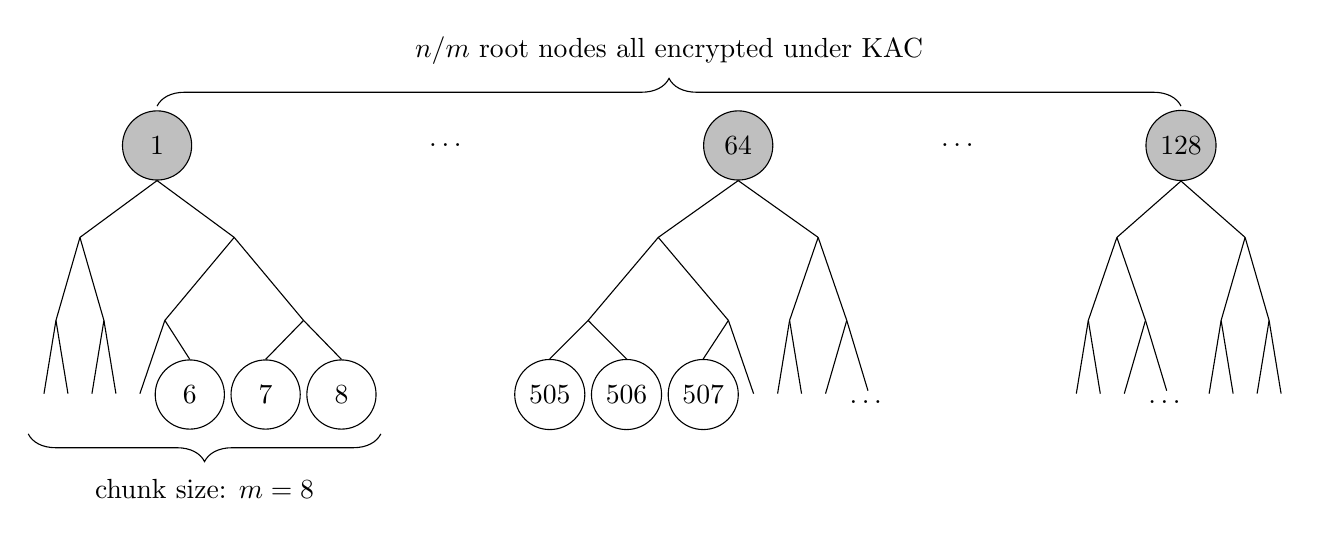
\begin{tikzpicture}


\tikzstyle{block} = [draw, circle, minimum size=2.5em]
\tikzset{level distance=30pt}

\begin{scope}[frontier/.style={distance from root=150pt},yshift=-50pt]
\Tree [.\node[draw, circle, fill=gray!50,minimum size=2.5em](root1){1}; 
[ [ [.\node(left-leaf) {}; ] [.{}  ]  ]
[  [.{}  ] [.{} ] ] ]
[  [ [.{}  ] [.\node[block] {6};    ] ]
[  [.\node[block] {7}; ] [.\node[block](right-leaf) {8}; ] ] ] ]
\end{scope}

\begin{scope}[frontier/.style={distance from root=150pt},xshift=210pt,yshift=-50pt]
\Tree [.\node[draw, circle, fill=gray!50, minimum size=2.5em](root2){64}; 
[ [ [.\node[block] {505}; ] [.\node[block] {506};  ]  ]
[  [.\node[block] {507};  ] [.{} ] ] ]
[  [ [.{}  ] [.{}   ] ]
[  [.{} ] [.{\dots} ] ] ] ]
\end{scope}

\begin{scope}[frontier/.style={distance from root=150pt},xshift=370pt,yshift=-50pt]
\Tree [.\node[draw, circle, fill=gray!50, minimum size=2.5em](root3){128};
[ [ [.{} ] [.{}  ]  ]
[  [.{}  ] [.{\dots} ] ] ]
[  [ [.{}  ] [.{}   ] ]
[  [.{} ] [.{} ] ] ] ]
\end{scope}

\begin{scope}
\draw [decorate,decoration={brace,amplitude=10pt},xshift=0pt,yshift=-5pt] ($(root1)+(0,0.5)$) -- ($(root3)+(0,0.5)$) node[midway,yshift=20pt]{$n/m$ root nodes all encrypted under KAC};
\draw [decorate,decoration={mirror, brace,amplitude=10pt},xshift=0pt,yshift=-150pt] ($(left-leaf |- right-leaf) + (-0.2,-0.5)$) -- ($(right-leaf) + (0.5,-0.5)$)node[midway,yshift=-20pt]{chunk size: $m=8$};
\end{scope}


\node at  ($ (root1) !.5! (root2) $) {\dots};
\node at  ($ (root2) !.5! (root3) $) {\dots};

\end{tikzpicture}
\caption{KAC-GGM hybrid structure}
\label{fig:kac-hash-tree}
\end{figure}

To release keys for $[6, 507]$, KG sends AU an KAC aggregate key $K_S, S=\{2,3,\dots,62,63\}$. This allows AU to decrypt GGM roots and derive the keys for $[9, 504]$. GGM roots $1,64$ are not included in $S$ as it will allow AU to derive keys outside of $[6,507]$. KAG builds the GGM tree and releases the inner nodes needed to derive the keys for $[6,8]$ and $[505,507]$, in a manner similar to GGM trees illustrated in \cref{fig:cover-ggm}.



\subsection{Variable Chunking}
\label{sec:mono-kac-ggm}

An alternate method of constructing the scheme explained in \cref{sec:kac-ggm} is to use a single GGM tree. As seen in \cref{fig:kac-ggm-monolithic}, KG first uses a GGM root node to derive $n$ leaf nodes. The monolithic tree is decomposed into $n/m$ subtrees, each subtree having $m$ leaf nodes. KG then encrypts the root node of each subtree under KAC, represented by the shaded nodes.
\begin{figure}[H]
\centering
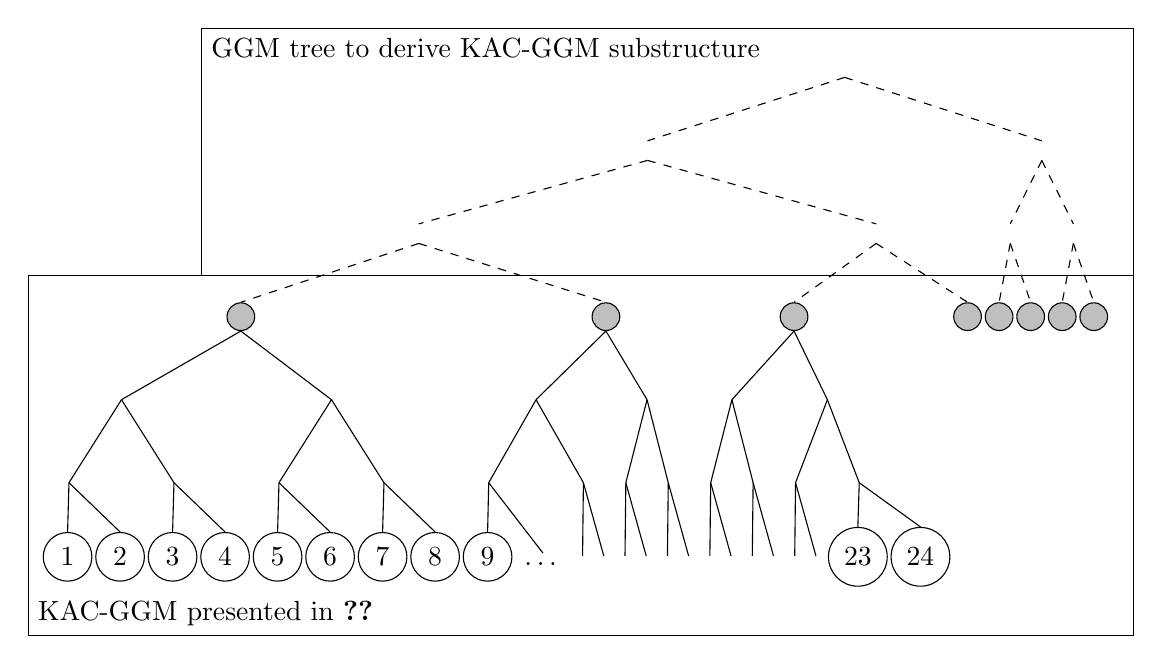
\begin{tikzpicture}


 % all changes only affect trees within this environment ,fill=
\tikzset{level distance=30pt,sibling distance=1pt}
\tikzset{every tree node/.style={anchor=base west}} % allign nodes of the tree to the left (west)

\Tree [ .\node(e){}; \edge[dashed];
[.{} \edge[dashed]; [.\node(before-kac){};   \edge[dashed];
[.\node[draw, circle, minimum size=1em, fill=gray!50](left-kac){}; [ [ [.\node[draw, circle, minimum size=1em](left-leaf){1}; ][.\node[draw, circle, minimum size=1em]{2}; ] ][ [.\node[draw, circle, minimum size=1em]{3}; ][.\node[draw, circle, minimum size=1em]{4}; ] ] ] [ [ [.\node[draw, circle, minimum size=1em]{5}; ][.\node[draw, circle, minimum size=1em]{6}; ] ] [  [.\node[draw, circle, minimum size=1em]{7}; ] [.\node[draw, circle, minimum size=1em]{8}; ] ] ] ]  \edge[dashed]; [.\node[draw, circle, minimum size=1em, fill=gray!50](y){};  [ [ [.\node[draw, circle, minimum size=1em]{9}; ][.{$\dots$} ] ][ [.{} ][.{} ] ] ] [ [ [.{} ][.{} ] ] [  [.{} ] [.{} ] ] ]  ]  ] \edge[dashed];
[ .{} \edge[dashed];  
[.\node[draw, circle, minimum size=1em, fill=gray!50]{}; [ [ [.{} ][.{} ] ][ [.{} ][.{} ] ] ] [ [ [.{} ][.{} ] ] [  [.\node[draw, circle, minimum size=1em]{23}; ] [.\node[draw, circle, minimum size=1em]{24}; ] ] ]  ]  \edge[dashed]; [.\node[draw, circle, minimum size=1em, fill=gray!50](start-subtree){}; ] ] ] \edge[dashed];
[.{} \edge[dashed]; [.{}  \edge[dashed];
[.\node[draw, circle, minimum size=1em, fill=gray!50]{}; ]  \edge[dashed]; [.\node[draw, circle, minimum size=1em, fill=gray!50]{};    ] ] \edge[dashed];
[.{} \edge[dashed];
[.\node[draw, circle, minimum size=1em, fill=gray!50]{}; ]  \edge[dashed]; [.\node[draw, circle, minimum size=1em, fill=gray!50](right-kac){};    ]  ] ] ]

\coordinate (pre-kac) at ($(left-kac)!0.5!(before-kac)$) ;
\draw[] ($(pre-kac -| left-kac) -(0.5,0)$) rectangle ($(right-kac |- e) +(0.5,0.5)$) ;
\draw[] ($(left-leaf) - (0.5,1)$) rectangle ($(right-kac |- pre-kac) + (0.5, 0)$) ;

\node[anchor=south west] at ($(left-kac |- e) + (-0.5,0)$ ) {GGM tree to derive KAC-GGM substructure} ;
\node[anchor=south west] at ($(left-leaf) - (0.5,1)$)  {KAC-GGM presented in~\cref{fig:kac-hash-tree}} ;

\end{tikzpicture}
\caption{Generalization of construction shown in \cref{fig:kac-hash-tree}}
\label{fig:kac-ggm-monolithic}
\end{figure}

Instead of using fixed size chunks, we are able to generalize the KAC-GGM construction to support variable chunking. We illustrate variable chunking with some examples. To decrypt $[1,1024]$, the ideal chunk size is $m=n=1024$. Only a single GGM node is required to generate all frame keys. To decrypt $[1, 522]$, we can divide the range into subranges $[1,512]$, $[513,520]$ and $[521, 522]$, yielding ideal chunk sizes $m_1=512, m_2=8, m_3=2$ respectively. Using such decomposition methods, AU only requires $3$ GGM nodes to derive $[1,512]$.



\begin{figure}[h]
\centering
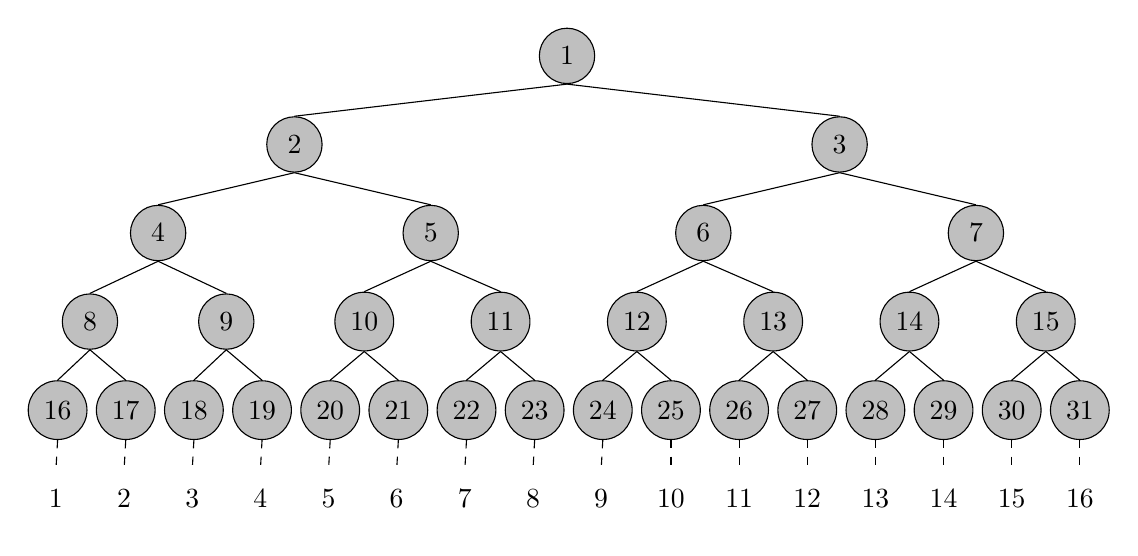
\begin{tikzpicture}
 % all changes only affect trees within this environment ,fill=
\tikzset{level distance=32pt,sibling distance=3pt}
\tikzset{every tree node/.style={anchor=base west, draw, circle, minimum size=2em, fill=gray!50}} % allign nodes of the tree to the left (west)
\begin{scope}
\Tree [ .{1} 
[.{2} 
[.{4}   
[.{8}  [.16 \edge[dashed]; \node[fill=none, draw=none]{1}; ] [.17 \edge[dashed]; \node[fill=none, draw=none]{2}; ] ] [.{9} [.18 \edge[dashed]; \node[fill=none, draw=none]{3}; ] [.19 \edge[dashed]; \node[fill=none, draw=none]{4}; ] ]  ]
[ .{5}  [.10 [.20 \edge[dashed]; \node[fill=none, draw=none]{5}; ] [.21 \edge[dashed]; \node[fill=none, draw=none]{6}; ] ] [.11 [.22 \edge[dashed]; \node[fill=none, draw=none]{7}; ] [.23 \edge[dashed]; \node[fill=none, draw=none]{8}; ] ]  ] ]
[.{3} [.{6}   [.12 [.24 \edge[dashed]; \node[fill=none, draw=none]{9}; ] [.25 \edge[dashed]; \node[fill=none, draw=none]{10}; ] ] [.13 [.26 \edge[dashed]; \node[fill=none, draw=none]{11}; ] [.27 \edge[dashed]; \node[fill=none, draw=none]{12}; ]]  ]
[.{7}   [.14 [.28 \edge[dashed]; \node[fill=none, draw=none]{13}; ] [.29 \edge[dashed]; \node[fill=none, draw=none]{14}; ] ] [.15 [.30 \edge[dashed]; \node[fill=none, draw=none]{15}; ] [.31 \edge[dashed]; \node[fill=none, draw=none]{16}; ] ]  ] ] ]


%\draw ($(b) + (1cm,1cm)) -- ($(c)!0.5!(d)$);
\end{scope}

\end{tikzpicture}
\caption{Generalized KAC-GGM (All GGM nodes are encrypted under KAC)}
\label{fig:kac-ggm-general}
\end{figure}

The construction for variable chunking is the same as described in \cref{fig:kac-ggm-monolithic} with a slight difference. Instead of encrypting only a single tree stratum, we now encrypt every node in the GGM tree, as shown in \cref{fig:kac-ggm-general}. Each shaded node is encrypted using its own unique KAC ciphertext class numbered in a breadth-first fashion. To release keys for for $[3,8]$, KG simply forwards $K_{\hat{S}}$, where $\hat{S}=\{9, 5\}$ to AU. AU uses $K_{\hat{S}}$ to decrypt nodes $9,5$. AU then decrypts node $9$ and node $5$ using KAC. After decryption of the GGM nodes, AU is able to reconstruct the GGM subtrees with node $9$ and $5$ as the root, deriving frame keys for $[3,4]$ and $[5,8]$ respectively. As compared to fixed chunking, variable chunking results in even lower granularity, which translates to higher decryption speeds.



\section{KAC Decryption Optimizations}

\label{sec:kac-range-decryption}

The construction of KAC's \textbf{Decrypt} algorithm provides a lot of opportunities for optimization. The decryption of a single ciphertext ($\mathfrak{C}_i$) under KAC is defined as:
\[
m_i = c_{i_3}  \, \cdot \,  \hat{e}(K_S \cdot   \prod_{j \in S, j \neq i} g_{n+1-j+i}, \, c_{i_1}) \, / \,  \hat{e}(  \prod_{j \in S} g_{n+1-j}, c_{i_2}) 
\]


%$\langle c_{i_1}, c_{i_2}, c_{i_3} \rangle$ are components of $\mathfrak{C}$$_i$. 
where $\mathfrak{C}_i = \langle c_{i_1}, c_{i_2}, c_{i_3} \rangle$. We denote $\displaystyle \rho_{i}=\prod_{j \in S, j \neq i} g_{n+1-j+i}$ and $\displaystyle \lambda = \prod_{j \in S} g_{n+1-j}$. 

\subsection{Decryption under same $K_S$}

For decryptions under the same $K_S$, the value of $\lambda$ remains unchanged as it is independent of $i$. $\lambda$ can be computed once and reused for subsequent decryptions instead of recomputing it for $Q$ times. This simple strategy can save a total of $|S|(|Q|-1)$ multiplications.

%Notice that for all decryptions under the same $S$ and $K_S$, $\hat{e} (\displaystyle  \prod_{j \in S} g_{n+1-j}, c_2)$ remains constant (denoted by $\beta$ for simplicity). As Bob is likely to decrypt a range of video frames at the same time, by precomputing and storing this value for a set of queries under the same aggregate key $K_S$, we are able to reduce the number of multiplications in the decryption of a single frame from $2|S|+1$ to $|S|$ and from 2 pairings to just a 1 pairing. 

\subsection{Optimization for varying frame rates}
\label{sec:kac-arithmetic}
In the KAC-GGM hybrid scheme presented in \cref{sec:kac-ggm-hybrid}, higher decryption speed is achieved by creating chunks of contiguous frames. However, the chunking strategy is not useful if we want to decrypt non-contiguous frames, especially frames which are part of an arithmetic sequence. Optimizing decryption for arithmetic sequences is especially useful if we want to support video decryption of varying frame rates. For instance, AU with limited access rights may only be allowed to decrypt the video only at $\frac{1}{8}$ of the original frame rate. This translates to the set of frames belonging to the arithmetic sequence, $a_i = a_1 + 8(i-1), i \geq 1$. We are able to speed up the computation of $\rho$ for arithmetic sequences and support fast decryption of varying frame rates.


Suppose $S$ and $Q$ are single arithmetic sequences where, ${S} = \{x, x+d, x+2d, \dots, x+d(|S|-1)\}, Q= \{i, i+d, i+2d, \dots, i+d(|Q|-1) \}, Q \subseteq {S}$.

For the the message encrypted under $i^{th}$ ciphertext class $(m_i)$, we have 
\begin{align*}
\displaystyle
\rho_{i} &= \prod_{j \in S, j \neq i } g_{n+1-j+i}\\
	&=(\prod^{|S|-1}_{j=0} g_{n+1-(x+jd)+i} )/ g_{n+1}
\end{align*}
To compute $m_{i+d}$, AU is able to make use of $\rho_i$.
\begin{align*}
\rho_{i+d} &= \prod_{j \in S, j \neq i+d } g_{n+1-j+(i+d)}\\
	&= (\prod^{|S|-1}_{j=0} g_{n+1-(x+jd)+(i+d)} )/ g_{n+1} \\
	&= \frac{g_{n+1-x + i + d} }{ g_{n+1-(x+d(|S|-1))+i}  \times g_{n+1}} \times \prod^{|S|-1}_{j=0} g_{n+1-(x+jd)+i}  \\
%	&= \frac{g_{n+1-x-(|S|-2)d+i} }{g_{n+1-x+i} \times g_{n+1}} \times \prod^{|S|-1}_{j=0} g_{n+1-(x+jd)+(i+d)}  \\
	&=  \frac{g_{n+1-x + i + d} }{ g_{n+1-(x+d(|S|-1))+i}} \times \rho_{i}
\end{align*}

AU then applies this optimization recursively for $\rho_{i+2d}, \rho_{i+3d}, \dots, \rho_{i+d(|Q|-1)}$ instead of recomputing $\rho$ each time. Substantial speedups have been observed from actual experiments. These results will be presented in \cref{sec:range-analyze}. 


\section{Homomorphic MAC}
\label{sec:homomophic}
One of the drawbacks of using KAC is the $\Theta(n)$ size \texttt{param} that is required to be stored in KG. In this section, we introduce a protocol that alleviates this issue, reducing the amount of private storage needed from $\Theta(n)$ to $O(1)$. 

The aggregate key is computed as $\displaystyle  K_S = \prod_{j \in S} g^{\gamma}_{n+1-j}$, where $\gamma$ is the \texttt{msk}. Hence, we are able to delegate the computation of  $\displaystyle \prod_{j \in S} g_{n+1-j}$ to the AU instead, especially since AU would have already obtained $\texttt{param} = \langle g, g_1, g_2, \dots, g_n, g_{n+2}, \dots, g_{2n} \rangle$ from RC which is required for running KAC's \textbf{Decrypt}. 

\begin{enumerate}
\item AU has rights to access frame keys of set $S$.
\item AU obtains \texttt{param} from RC.
\item AU computes and submits $\langle \displaystyle \prod_{j \in S} g_{n+1-j}, S \rangle$ to KG.
\item KG verifies that AU is entitled to frames of set $S$.
\item KG computes $K_S = \displaystyle \prod_{j \in S} g^{\gamma}_{n+1-j} = (\displaystyle \prod_{j \in S} g_{n+1-j})^\gamma$.
\item KG transfers $K_S$ to AU.
\item AU uses $K_S$ and \texttt{param} to decrypt the frames in $S$.
\end{enumerate}

With such a verification protocol, there is no need for KG to store the linear-size \texttt{param} as part of the computation of $K_S$ is delegated to AU. KG is only responsible for exponentiating the product of the group elements in \texttt{param} with \texttt{msk}. However, this scheme is vulnerable to spoofing attacks, as there is no way for the server to verify AU's computation.

Consider Harry, a malicious AU, who only has authorized access to keys in set $S$. He is however interested in obtaining keys in set $U$, $U \not\subseteq S$. 

\begin{enumerate}
\item Harry computes and sends KG $\langle \displaystyle \prod_{j \in U} g_{n+1-j}, S \rangle$.
\item KG verifies that Harry have access to $S$.
\item KG computes and transfers $K_{U} = \displaystyle (\prod_{j \in U} g_{n+1-j})^{\gamma}$ to Harry.
\item Harry has managed to convince the server to $K_U$. Using $K_U$, he is able to generate frame keys in $U$ which he does not have the authority to access.
\end{enumerate}

To prevent such attacks, KG needs to be able to verify AU's computation to ensure that it is indeed $\displaystyle \prod_{j \in S} g_{n+1-j}$ and not a spoofed value.

\subsection{Verification Protocol}
\label{sec:verify}
In order to verify AU's computation, we introduce a protocol based on homomorphic MAC construction which allows KG to verify the AU's computation without the need to store \texttt{param}. The protocol consists of 3 algorithms, \textbf{Signing}, \textbf{Computation}, \textbf{Verification}.


\paragraph{Signing} DO signs the group elements in \texttt{param} which used to generate the aggregate key, $K_S$. We denote this set of signatures as \texttt{param\_sig}.
\begin{enumerate}
\item DO select random values $\beta, \beta_1, \beta_2, \dots, \beta_n \in \mathbb{Z}_{p}$.
\item DO extracts $n+1$ group elements $g, g_1, \dots, g_n$ from \texttt{param}. $g$ is the generator for $\mathbb{G}$, while $g_1, g_2, \dots , g_n$ are the group elements used in the computation of $K_S$. 
\item DO computes $\texttt{param\_sig} = \langle g_1^{\beta}  g^{\beta_1}, g_2^{\beta}  g^{\beta_2}, \dots, g_n^{\beta}  g^{\beta_n} \rangle = \langle a_1, a_2, \dots, a_n \rangle$, the homomorphic signature for $\langle g_1, \dots , g_n \rangle$.
%\item DO uploads $\texttt{param\_sig}$, $\texttt{param}$  to RC.
%\item DO transfers $\beta, \beta_1, \beta_2, \dots, \beta_n$ and $g$ to KG.
\end{enumerate}


\paragraph{Computation} AU computes the necessary parameters required for the generation for an aggregate key and forwards it to KG. 

\begin{enumerate}
\item AU has access rights to frame keys of set $S$.
\item AU obtains \texttt{param} and \texttt{param\_sig} from RC.
\item AU computes and submits $\langle w_1, w_2, w_3 \rangle = \displaystyle \langle \displaystyle \prod_{i \in S} g_{n+1-i} \, , \, \prod_{i \in S} a_{n+1-i}, S\rangle$ to KG. 
%$\prod_{i \in S} a_{n+1-i}$ serves as a proof that AU indeed has performed $\prod_{i \in S} g_{n+1-i}$.

\end{enumerate}

\paragraph{Verification} KG verifies $\langle w_1, w_2, w_3 \rangle$. $K_S$ is issued only if $w_1,w_2$ are computed using the elements in \texttt{param} and \texttt{param\_sig} corresponding to set $w_3$.
\begin{enumerate}
\item KG computes $\texttt{aggregate\_sig} = \displaystyle w_1^{\beta} \times \prod_{i \in w_3}  g^{\beta_{n+1-i}}$.
\item KG computes the $K_{w_3} = w_1^\gamma$ only if $\texttt{aggregate\_sig} =  w_2$.
\end{enumerate}

This scheme still requires DO to send $\beta, \beta_1, \beta_2, \dots, \beta_n$ to KG, consuming $\Theta(n)$ bandwidth. Instead of storing them permanently, DO could choose to generate $\beta_1, \beta_2 \dots \beta_n$ using a random oracle from $\beta$. Therefore, DO only has to send constant-size $\beta$ to KG. KG can then derive $\beta_1, \beta_2 \dots \beta_n$ from $\beta$. A security proof of the protocol will be presented in \cref{sec:proof}.



\section{Provisioning for Layered Content}
\label{sec:layered}


It has become increasingly common for video files to be encoded with different resolutions. This strategy is commonly employed in video streaming sites to cater to clients with varying network bandwidth. In our case, different AUs are granted access rights to footage of different resolutions.  In this section, we explore mechanisms that support such capabilities.

We consider a video file with two quality levels, high quality (HQ) and low quality (LQ). Borrowing the ideas from \cref{chapt:mcp-abe}, we can segment the video into two layers, a LQ layer and a HQ enhancement layer. LQ video frames correspond to the LQ layer. To obtain HQ video frames, AU will need a combination of data from both LQ and HQ enhancement layer. In other words, the HQ enhancement layer contains information which is present in HQ frames but missing in LQ frames. This use of an enhancement layer reduces the amount of storage needed as there is no duplication of information between LQ and HQ frames. The HQ enhancement layer is higher in privilege compared to LQ layer, denoted as $HQ>LQ$.

%Both HQ and LQ frame keys are required to decrypt high resolution frames. Only LQ frame keys are needed to decrypt low resolution frames. AU with access to frame keys in HQ layer will be able to access frame keys in LQ layer since HQ is of higher privilege than LQ, denoted as $HQ>LQ$. 
%We are able segment the video into multiple layers with different privileges described in MCP-ABE in

\begin{figure}[h]
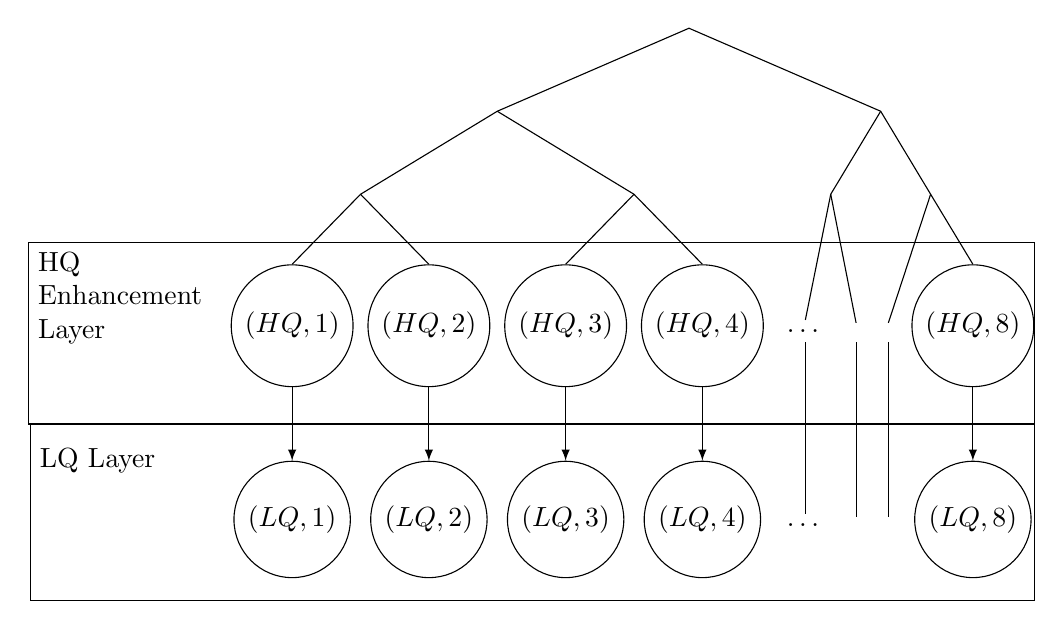
\begin{tikzpicture}
\tikzset{level 3/.style={level distance=50pt}}
\tikzset{level 4/.style={level distance=70pt}}
\tikzset{sibling distance=0.5em}
\Tree [ 
[ [ [.\node[draw,circle](HQ1){$(HQ,1)$}; \edge[-latex];[.\node[draw,circle](LQ1){$(LQ,1)$}; ] ] [.\node[draw,circle]{$(HQ,2)$}; \edge[-latex];[.\node[draw,circle]{$(LQ,2)$}; ] ]  ]
[ [.\node[draw,circle]{$(HQ,3)$}; \edge[-latex];[.\node[draw,circle]{$(LQ,3)$}; ] ] [.\node[draw,circle]{$(HQ,4)$}; \edge[-latex]; [.\node[draw,circle]{$(LQ,4)$}; ] ] ] ]
[  [ [.{$\dots$} [.{$\dots$} ] ] [.{} [.{} ] ] ]
[  [.{} [.{} ] ] [.\node[draw,circle](HQ8){$(HQ,8)$};  \edge[-latex]; [.\node[draw,circle](LQ8){$(LQ,8)$}; ] ] ] ] ]

%\path (HQ)  ++(50pt,0) node[anchor=west](HQ-text){HQ Enhancement Layer};
%\path (LQ)  ++(50pt,0) node[anchor=west](LQ-text){LQ Layer};
%
%
%\draw[latex-] (LQ-text) -- (LQ);
%\draw[latex-] (HQ-text) -- (HQ);
\coordinate(mid) at ($(HQ8.south)!0.5!(LQ1.north)$);
\draw ($(HQ1.north west) + (-2.8,0.5)$) rectangle (mid -| current bounding box.east)  ;
\node[anchor= north west, align=left] at  ($(HQ1.north west) + (-2.8,0.5)$) {HQ\\Enhancement\\Layer};
%\node at  ($ (root2) !.5! (root3) $) {\dots};
\draw ($(LQ1.south west) + (-2.8,-0.5)$) rectangle (mid -| current bounding box.east) ;
\node[anchor= north west] at  ($(LQ1.north west) + (-2.8,0.5)$) {LQ Layer};
\end{tikzpicture}
\caption{Layered hashing}
\label{fig:kac-layer}
\end{figure}



\cref{fig:kac-layer} features a combination of KAC-GGM with hash chaining which is described in \cref{chapt:mcp-abe} and Equation \ref{eq:hash-chain}. AU has access rights to frame keys $[(HQ, 1), (HQ,8)]$. Since $HQ>LQ$, AU is able to retrieve keys in $[(LQ, 1),(LQ,8)]$ by computing $(LQ,i) = h((HQ,i)||\text{padding})$, where $h$ is a hash function and $i$ represents the frame number, $1 \leq i \leq n$. By hashing the keys in the upper layer, AU is able to obtain the corresponding keys in the lower layers.

%Supposed Charlie is only entitled to LQ video from frames 2 to 4. Any inner nodes in the hash tree will inevitably leak keys belong to HQ Enhancement Layer which Charlie does not have access to. Since Charlie is unable to access any of the inner nodes of the tree, it is evident that the use of hash chaining is incompatible with hash tree.

Now suppose that AU only has access to $[(LQ, 1), (LQ,8)]$. It is clear from the \cref{fig:kac-layer} that we are unable to aggregate the LQ frame keys under the root as doing so exposes HQ frame keys. Consequently, decryption of the LQ layer can only be performed at the leaves of the tree which is highly inefficient. In fact, all layers except the highest privileged layer have to be decrypted at the leaves.  Hence, hash chaining is not a viable construction for encryption of layered content.

\subsection{Layered Symmetric Encryption}

A simple approach to support layered decryption is to generate $l$ KAC-GGM hybrid trees, $1$ tree for each layer. To decrypt $l$ layers, the AU runs KAC-GGM hybrid algorithm $l$ times. However, running KAC's \textbf{Decrypt} algorithm $l$ times can be slow.

Instead of using KAC to decrypt each layer, we can instead choose to use symmetric decryption to generate the frame keys for the lower layers, at a cost of additional public storage in RC. In addition to generating $l$ KAC-GGM hybrid structures, DO also encrypts the frame keys of layer $(i-1)$ using the frame keys of layer $i$ as the symmetric key, where $i$ represents the privilege level. 

For $l$ layers, we have $E_{k_{(i+1,j)}}(k_{(i,j)}), 1 \leq i \leq l, 1 \leq j \leq n$, where  $j$ represents frame number and $i$ represents the privilege level. This process gives us $l-1$ intermediate layers. Decrypting all $l$ layers involves KAC decryption of the highest layer, followed by symmetric decryption of $l-1$ intermediate layers. 

%
%We proposed a scheme which uses symmetric encryption to derive frame keys in the lower layers. DO generates a KAC structureBy encrypting the frame keys of lower layers with  of the  symmetric-key algorithm such as DES or AES, 
%



\begin{figure}
\centering

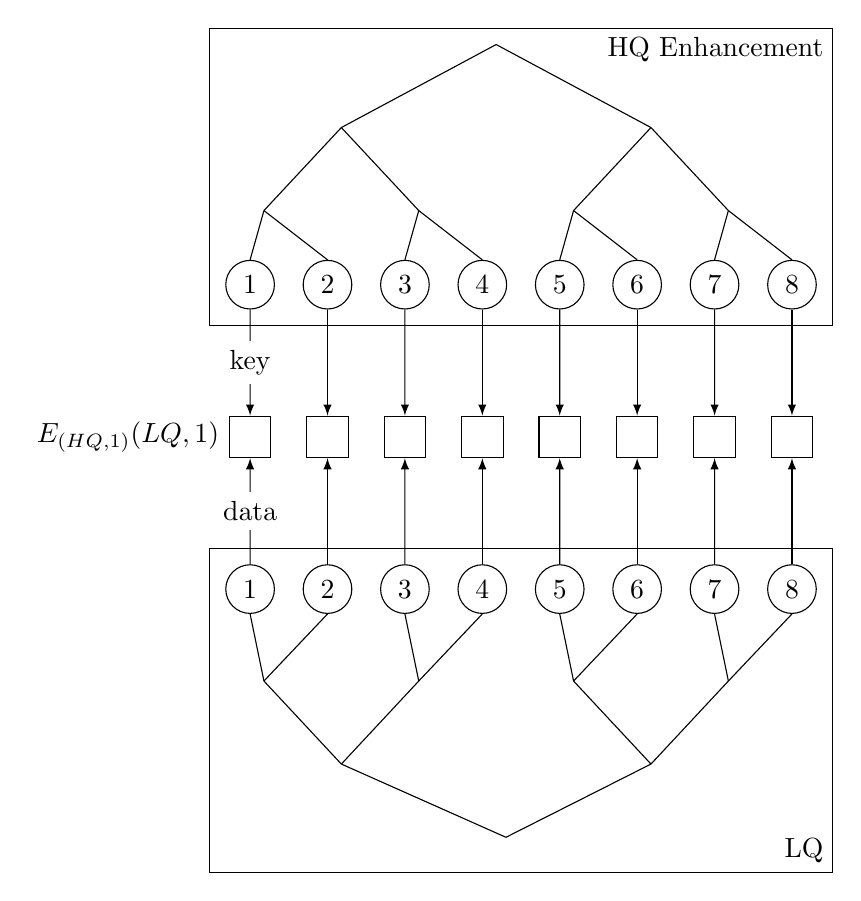
\begin{tikzpicture}
 % all changes only affect trees within this environment ,fill=
\tikzset{level distance=30pt,sibling distance=1em}
\tikzset{every tree node/.style={anchor=base west}} % allign nodes of the tree to the left (west)
\begin{scope}[frontier/.style={distance from root=100pt}]
\Tree [ 
[ 
[ [.\node[draw, circle, minimum size=1em](HQ1){1}; ][.\node[draw, circle, minimum size=1em](HQ2){2}; ] ] [ [.\node[draw, circle, minimum size=1em](HQ3){3}; ][.\node[draw, circle, minimum size=1em](HQ4){4}; ]] ]
[ 
[ [.\node[draw, circle, minimum size=1em](HQ5){5}; ][.\node[draw, circle, minimum size=1em](HQ6){6}; ]][ [.\node[draw, circle, minimum size=1em](HQ7){7}; ][.\node[draw, circle, minimum size=1em](HQ8){8}; ] ] 
] ]

\coordinate (northeast) at (current bounding box.north east);
\coordinate (southwest) at (current bounding box.south west);
\coordinate (southeast) at (current bounding box.south east);
\draw ($(northeast)+(0.2,0.2)$) rectangle ($(southwest)+(-0.2,-0.2)$) ;
\node[anchor=north east] at (current bounding box.north east) {HQ Enhancement};
%\coordinate (z) at ($(x)!0.5!(b)$) ;
%\draw[] ($(z -| b) -(0.5,0)$) rectangle ($(f |- e) +(0.5,0.5)$);
%\draw ($(b) + (1cm,1cm)) -- ($(c)!0.5!(d)$);
\end{scope}

\begin{scope}[frontier/.style={distance from root=100pt}, yshift=-290pt, grow'=up,draw, local bounding box=bb]
%\draw ($(local bounding box.north east)+(0.2,0.2)$) rectangle ($(local bounding box.south west)+(-0.2,-0.2)$) ;
\Tree [.\node(rootLQ){}; 
[ 
[ [.\node[draw, circle, minimum size=1em](LQ1){1}; ][.\node[draw, circle, minimum size=1em](LQ2){2}; ] ] [ [.\node[draw, circle, minimum size=1em](LQ3){3}; ][.\node[draw, circle, minimum size=1em](LQ4){4}; ]] ]
[
[ [.\node[draw, circle, minimum size=1em](LQ5){5}; ][.\node[draw, circle, minimum size=1em](LQ6){6}; ]][ [.\node[draw, circle, minimum size=1em](LQ7){7}; ][.\node[draw, circle, minimum size=1em](LQ8){8}; ] ] 
] ]

\draw ($(northeast|-LQ8.north) + (0.2,0.2)$) rectangle ($(southwest|-rootLQ.south)+(-0.2,-0.2)$) ;

\node[anchor=south east] at (current bounding box.south east) {LQ};
\end{scope}
%\coordinate (sym1) at ($(LQ1)!0.5!(HQ1)$); 
%\node[draw] at ($(HQ1) + (0,-1.7)$) (test) {lol};
%\node[] at ($(LQ1) + (0,-2.5)$) (test2) {lol};
%\draw[-latex] (LQ1) -- (test2) -- (test|-test2) -- (test);
\node[draw, minimum size=1.5em] at ($(HQ1)!0.5!(LQ1)$) (e1) {};
\node[anchor=east](test) at (e1.west) {$E_{(HQ,1)}(LQ,1)$} ;
\draw[-latex] (LQ1.north) -- (e1) node [fill=white,midway] {data};
\draw[-latex] (HQ1.south) -- (e1) node [fill=white,midway] {key};

\node[draw, minimum size=1.5em] at ($(HQ2)!0.5!(LQ2)$) (e2)  {};
\draw[-latex] (LQ2.north) -- (e2);
\draw[-latex] (HQ2.south) -- (e2);

\node[draw, minimum size=1.5em] at ($(HQ3)!0.5!(LQ3)$) (e3)  {};
\draw[-latex] (LQ3.north) -- (e3);
\draw[-latex] (HQ3.south) -- (e3);

\node[draw, minimum size=1.5em] at ($(HQ4)!0.5!(LQ4)$) (e4)  {};
\draw[-latex] (LQ4.north) -- (e4);
\draw[-latex] (HQ4.south) -- (e4);

\node[draw, minimum size=1.5em] at ($(HQ5)!0.5!(LQ5)$) (e5)  {};
\draw[-latex] (LQ5.north) -- (e5);
\draw[-latex] (HQ5.south) -- (e5);

\node[draw, minimum size=1.5em] at ($(HQ6)!0.5!(LQ6)$) (e6)  {};
\draw[-latex] (LQ6.north) -- (e6);
\draw[-latex] (HQ6.south) -- (e6);

\node[draw, minimum size=1.5em] at ($(HQ7)!0.5!(LQ7)$) (e7)  {};
\draw[-latex] (LQ7.north) -- (e7);
\draw[-latex] (HQ7.south) -- (e7);

\node[draw, minimum size=1.5em] at ($(HQ8)!0.5!(LQ8)$) (e8)  {};
\draw[-latex] (LQ8.north) -- (e8);
\draw[-latex] (HQ8.south) -- (e8);


%\draw ($(southeast)+ (0.2,-0.2)$) rectangle ($(test.west|-LQ8.north) + (-1.5,0.2)$) ;
%\node[anchor=south] at ($(test.west|-LQ8.north) + (0.2,0.2)$){Intermediate Layer};
%\draw[] ($(z -| b) -(0.5,0)$) rectangle ($(f |- e) +(0.5,0.5)$);
%\draw ($(b) + (1cm,1cm)) -- ($(c)!0.5!(d)$);


\end{tikzpicture}
\caption{Layered encryption using intermediate layers}
\label{fig:encrypt-chain}
\end{figure}

An example involving just $2$ layers is shown in \cref{fig:encrypt-chain}. LQ frame keys are encrypted by the frame keys of the HQ layer, forming an intermediate encrypted layer. For instance for frame $1$, $(LQ,1)$ is encrypted with using $(HQ,1)$ as the symmetric key, forming $E_{(HQ,1)}(LQ,1)$. The intermediate layer is stored in the RC along with the KAC. To obtain high resolution frames in range $[2,4]$, AU first derives keys in $[(HQ, 2),(HQ,4)]$ using KAC. AU then uses symmetric decryption to obtain $[(LQ, 2),(LQ,4)]$. 



%Extending this to $l$ is straightforward. 
%
%This scheme requires $l$ KAC structures and $l-1$ intermediate layers. A monolithic KAC-GGM (\cref{sec:mono-kac-ggm}) with $\phi=1$ and $l$ layers would result in RC storage overhead of $l*O(2n-1) + (l-1)n = O(ln)$. Since each layer is encrypted with a different KAC master key, KG has a storage overhead of $l * O(1) = O(l)$. reviewing our system model~\cref{chap:model} and

\chapter{Analysis}
\label{chap:analysis}
In this chapter, we present storage, runtime, as well as security analysis of our proposed techniques in \cref{sec:kac-ggm-runtime,sec:range-analyze,sec:homo-analyze,sec:layer-analyze}. In \cref{sec:summary}, we will look at how our proposed techniques can be applied to our model to fulfill performance and security requirements. Similar to \cref{chap:prelim}, experiments are performed on prototypes built using Charm~\cite{charm13} cryptographic framework, running on Macbook Air 2013 (Intel Core-i7-4650u). Symmetric pairings over Type-A (supersingular) curves with a base field of 512 bits are chosen as the underlying pairing group for KAC. For the implementation of GGM trees, SHA-256 was used as the underlying CSB, where $G_0(x) = \text{SHA-256}(x \, || \, $`$l$'$)$ and $G_1(x) = \text{SHA-256}(x \, || \, $`$r$'$)$. 

\section{KAC-GGM Hybrid}
\label{sec:kac-ggm-runtime}
In this section, we evaluate the runtime and storage performance of both fixed and variable chunking in a KAC-GGM hybrid scheme.

\subsection{Fixed Chunking}

\begin{table}[h]
    \begin{tabular}{|l|l| p{0.4\textwidth} | l |}
  \hline
    ~              & KAC                        & Fixed Chunking                                                               & Entity   \\ \hline
    $\mathfrak{C}$    & $\Theta(n)$ group elements & $\Theta(n/m)$ group elements                                           & RC       \\ \hline
    \texttt{param} & $2n$ group elements        & $2n/m$ group elements                                                  & RC, KG   \\ \hline
    GGM Root       & -                          & $n/m$ hash digests                                                     & KG       \\ \hline
    Meta-key       & $O(1)$                     & Contiguous $S$: $O(1) + 2\,O(\log(m))$ \newline Non-contiguous $S$: $O(|S|)$ & KG $\to$ AU \\ \hline
    \end{tabular}
    \caption{Storage comparison between KAC and KAC-GGM (Fixed Chunking)}
    \label{tab:kac-ggm-storage}
\end{table}


In \cref{tab:kac-ggm-storage}, we see that for contiguous decryption, KAC-GGM incurs a meta-key size of $O(1) + 2 \, O(\log(m))$. $O(1)$ being the size of the aggregate key $K_S$ and $2 \, O(\log(m))$ being the extra key material derived from the GGM tree in the start and end of the range, as illustrated in \cref{fig:kac-hash-tree}.

%For non-contiguous decryption, the situation is similar to GGM tree described in \cref{sec:ggm}. None of the keys can be aggregated and the KG will have to send $O(n)$ leaf nodes to AU.   
For non-contiguous decryption, none of the keys can be aggregated. Therefore, KG has to send $O(n)$ leaf nodes to AU.  

The total amount of storage required by RC has been reduced from $\Theta(n)$ to $\Theta(n/m)$ due to the reduction in ciphertext classes. The storage requirements of KG on the other hand, have changed from $2n$ group elements to $2n/m$ group elements and $n/m$ hash digests. Since $m \geq 2$, there is a net reduction of storage in KG.


Empirical results in \cref{fig:kac-ggm-encrypt-decrypt} show that running time of encryption exhibits linear speedup with respect to increasing $m$. Contiguous decryption complexity for fixed chunking is calculated to be $(|Q|/m) \, \Theta(|S|/m) = O(|S|^2/m^2)$. The plot has a gradient of $-2$ for $m \leq 2^7$. This translates to a speedup of $m^2$, consistent with our theoretical calculations. For $m>2^7$, runtime gains are sub-optimal. This can be attributed to GGM tree generation dominating over the runtime of KAC decryption.
\begin{figure}[H]
\centering

\begin{subfigure}[t]{0.5\textwidth}
\begin{tikzpicture}

\begin{loglogaxis}[xlabel={$m$},width=1\linewidth,ylabel={Time (s)}, legend pos=north east,  title={$n=65536$, $Q=S$, Contiguous $Q$, $|Q| = 32768$ }]

%\addplot+[mark=x, smooth]  table[x index=0,y index=1,col sep=comma] {../Code/SS1024/kac_layer_encrypt_time.csv};
%\addplot+[smooth] table[x index=0,y index=1,col sep=comma] {../Code/SS1024/kac_layer_decrypt_time.csv};
\addplot+[smooth]  table[x index=0,y index=1,col sep=comma] {../Code/SS512/kac_layer_encrypt_time.csv};
\addplot+[smooth] table[x index=0,y index=1,col sep=comma] {../Code/SS512/kac_layer_decrypt_time_2.csv}
coordinate [pos=0] (A)
   coordinate [pos=0.65]  (B);;


   
\draw (A) -| (B);
\node[anchor=south west] at ($(B)!0.5!(A)$) {$-2$};

%\addlegendentry{Encryption (SS1024)}% y index+1 since humans count from 1
%\addlegendentry{Decryption (SS1024)}% y index+1 since humans count from 1
\addlegendentry{Encryption}% y index+1 since humans count from 1
\addlegendentry{Decryption}% y index+1 since humans count from 1




\end{loglogaxis}
\end{tikzpicture}
\caption{KAC-GGM Encrypt/Decrypt Time}
\label{fig:kac-ggm-encrypt-decrypt}
\end{subfigure}~
\begin{subfigure}[t]{0.5\textwidth}
\begin{tikzpicture}

\begin{loglogaxis}[xlabel={$|Q|$},width=1\linewidth,ylabel={Time (s)}, legend pos=north west, title={$Q=S$, Contiguous $Q$}]

\addplot+[smooth]  table[x index=0,y index=1,col sep=comma] {../Code/SS512/kac_normal_decrypt_time.csv};
\addplot+[smooth] table[x index=0,y index=1,col sep=comma] {../Code/SS512/kac_layer_decrypt_time_m64_2.csv};
\addlegendentry{m=1, no GGM}% y index+1 since humans count from 1
\addlegendentry{m=64}% y index+1 since humans count from 1
\end{loglogaxis}
\end{tikzpicture}
\caption{KAC-GGM Decryption Speedup}
\label{fig:kac-ggm-speedup}
\end{subfigure}
\caption{Empirical results of KAC-GGM}

\end{figure}

\cref{fig:kac-ggm-speedup} compares a specific case of $m=64$ and original KAC. A speedup from $O(|S|^2)$ to $O((|S|/2^6)^2) = O(|S|^2/2^{12})$ is observed for $|S| \geq 2^{14}$.





\subsection{Variable Chunking}

In variable chunking where all GGM nodes are encrypted under KAC, the amount of KAC ciphertext increases from $n$ to $2n-1$. Hence, the storage required for \texttt{param} and $\mathfrak{C}$ will be twice of that of a normal KAC scheme (\cref{sec:kac-private,sec:kac-public}). As every node is encrypted with KAC, KG is able to issue a constant-size KAC aggregate-key for any combination of nodes. Hence, the meta-key is always $O(1)$ in size. $O(\log(n))$ nodes is sufficient to represent any contiguous range. Therefore, using KAC's \textbf{Decrypt} algorithm together with variable chunking will require only $O(\log^2(n))$ decryption time at most. In our experiments shown in \cref{fig:kac-ggm-graph}, variable chunking demonstrated short runtimes even for large datasets, much faster than realtime requirements of 24FPS. Variable chunking KAC-GGM hybrid scheme managed to generate all frame keys under $1$ sec even for datasets as large as $|S|=2^{14}$.

\begin{figure}
\centering
\begin{tikzpicture}

\begin{loglogaxis}[xlabel={$|S|$},width=0.8\textwidth,ylabel={Time (s)}, legend pos=north west, title={$Q=S$, contiguous $Q$}]
\addplot+[smooth] table[x index=0,y index=1,col sep=comma] {../Code/SS512/kac_normal_decrypt_time.csv};
\addplot+[smooth, mark=x] table[x index=0,y index=1,col sep=comma] {../Code/SS512/mono_decrypt_time_fine.csv};
%\addplot+[smooth] table[x index=0,y index=1,col sep=comma] {../Code/SS512/kac_range_decrypt_time.csv};


\addplot+[no markers, domain=1:32768, dashed]{x/24};
%\addplot+[no markers, domain=1:32768, dotted, thick, black]{x/72};

\addlegendentry{Original KAC}
\addlegendentry{Monolithic}
\addlegendentry{24 FPS}
\end{loglogaxis}
\end{tikzpicture}
\caption{Monolithic KAC-GGM decryption time}
\label{fig:kac-ggm-graph}
\end{figure}




Despite the huge improvements in runtime, the significant increase in storage costs incurred by KG and RC is undesirable. Instead of encrypting all stratum in the GGM tree, DO may opt to skip and encrypt only specific strata in the tree. In the example shown in \cref{fig:kac-ggm-general-gap1}, nodes are encrypted once every $2$ strata $(\phi = 2)$. 



\begin{figure}
\centering
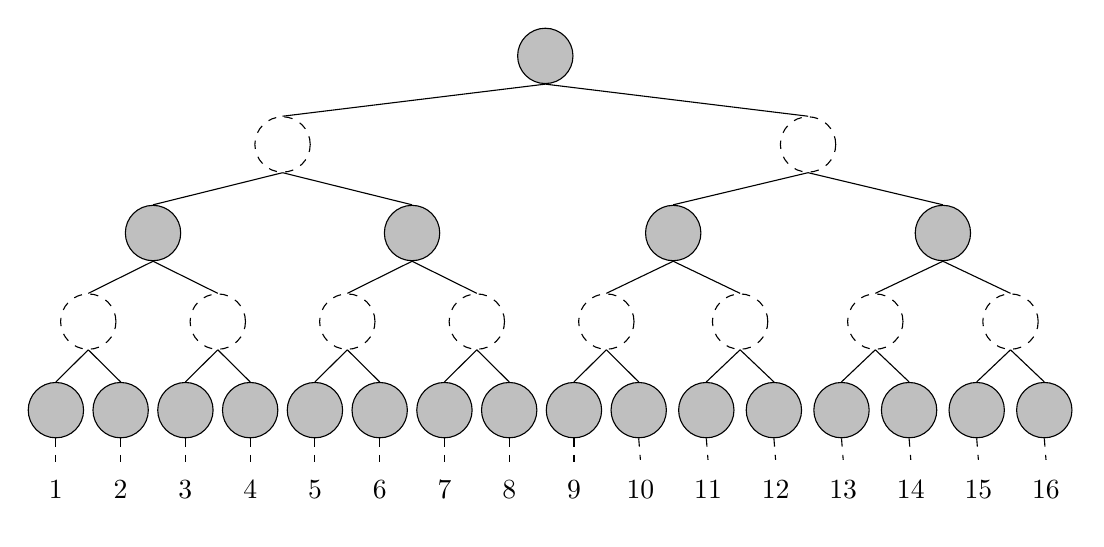
\begin{tikzpicture}
\tikzstyle{skip} = [fill=none,draw, circle, dashed]  
 % all changes only affect trees within this environment ,fill=
\tikzset{level distance=32pt,sibling distance=3pt}
\tikzset{every tree node/.style={anchor=base west, draw, circle, minimum size=2em, fill=gray!50}} % allign nodes of the tree to the left (west)
\begin{scope}
\Tree [ .{} 
[.\node[skip] {}; 
[.{}   
[.\node[skip] {};   [.{} \edge[dashed]; \node[fill=none, draw=none]{1}; ] [.{} \edge[dashed]; \node[fill=none, draw=none]{2}; ] ] [.\node[skip] {};  [.{} \edge[dashed]; \node[fill=none, draw=none]{3}; ] [.{} \edge[dashed]; \node[fill=none, draw=none]{4}; ] ]  ]
[ .{}  [.\node[skip] {};  [.{} \edge[dashed]; \node[fill=none, draw=none]{5}; ] [.{} \edge[dashed]; \node[fill=none, draw=none]{6}; ] ] [.\node[skip] {};  [.{} \edge[dashed]; \node[fill=none, draw=none]{7}; ] [.{} \edge[dashed]; \node[fill=none, draw=none]{8}; ] ]  ] ]
[.\node[skip] {}; [.{}   [.\node[skip] {};  [.{} \edge[dashed]; \node[fill=none, draw=none]{9}; ] [.{} \edge[dashed]; \node[fill=none, draw=none]{10}; ] ] [.\node[skip] {};  [.{} \edge[dashed]; \node[fill=none, draw=none]{11}; ] [.{} \edge[dashed]; \node[fill=none, draw=none]{12}; ]]  ]
[.{}   [.\node[skip] {};  [.{} \edge[dashed]; \node[fill=none, draw=none]{13}; ] [.{} \edge[dashed]; \node[fill=none, draw=none]{14}; ] ] [.\node[skip] {};  [.{} \edge[dashed]; \node[fill=none, draw=none]{15}; ] [.{} \edge[dashed]; \node[fill=none, draw=none]{16}; ] ]  ] ] ]


%\node at ( $((left-kac)!0.5!(before-kac)) + (-0.5,0)$ ) {GGM to derive KAC nodes} ;

%\draw ($(b) + (1cm,1cm)) -- ($(c)!0.5!(d)$);
\end{scope}

\end{tikzpicture}
\caption{Generalized KAC-GGM with $\phi = 2$}
\label{fig:kac-ggm-general-gap1}
\end{figure}



Leaving gaps and encrypting once every $\phi$ strata will reduce the number of encrypted nodes from $2n -1$ to $(2^{\phi} \, n - 1) / (2^{\phi} -1)$, reducing storage required in RC. However, this comes at the expense of decryption efficiency since more nodes now are required to represent a contiguous range of values. The number of nodes is needed to represent a single range is increased from $O(\log(n))$ to $O(2^{\phi} + \log(n))$.



\section{KAC Decryption Optimization}
\label{sec:range-analyze}
In this section, we analyze the asymptotic and empirical runtimes of KAC decryption optimizations discussed in \cref{sec:kac-range-decryption}. A comparison of decryption complexities and number of operations needed for various algorithmic optimizations is presented in \cref{tab:kac-optimize}.

\begin{table}[H]
\renewcommand{\arraystretch}{1.2}
    \begin{tabularx}{\textwidth}{| p{0.20\textwidth} | >{\raggedright\let\newline\\\arraybackslash\hspace{0pt}}X | >{\raggedright\let\newline\\\arraybackslash\hspace{0pt}} p{0.15\textwidth} | >{\raggedright\let\newline\\\arraybackslash\hspace{0pt}} p{0.15\textwidth} | >{\raggedright\let\newline\\\arraybackslash\hspace{0pt}}X |}
  
    \hline
    ~               & Multiplication & Pairing & Division   & Total                  \\ \hline
    Unoptimized KAC  & $|Q|(2|S|+1)$         & $2|Q| $          & $|Q|$           & $2|Q||S|+\Theta(|Q|)$       \\ \hline
    $\lambda$ reuse & $|Q|(|S|+1) + |S|$         & $2|Q| $          & $|Q|$           & $|Q||S|+\Theta(|Q|)+\Theta|S|$       \\ \hline    
    $\lambda, \rho_{i}$ reuse     & $3|Q| +2|S| -2$ & $2|Q|$         & $2|Q| - 1$  & $7|Q| + 2|S| - O(1)$ \\ \hline
    KP-ABE             &  $|Q|O(\log(n))$         & $|Q|O(\log(n))$   & $|Q|O(\log(n))$      & $|Q|O(\log(n))$                  \\ \hline
    
  \end{tabularx}

    \caption{Decryption complexity (Contiguous $S,Q$, arithmetic sequences of $d=1$)}
        \label{tab:kac-optimize}
\end{table}


For arithmetic sequences, $Q=S$, reusing $\rho_i$ results in asymptotic runtime improvement from $\Theta(|S|^2)$ to $\Theta(|S|)$.  Experimental results in \cref{fig:kac-abe-decrypt-optimize} showed that decryption for arithmetic sequences are much faster than KP-ABE as well as realtime requirements of 24FPS. 

\begin{figure}[H]
\centering
\begin{tikzpicture}

\begin{loglogaxis}[width=0.8\textwidth, xlabel={$|Q|$},ylabel={Time (s)}, title={Decryption Time. $n=65536, Q=S, \text{Contiguous } Q$}]


\addplot+[smooth] table[x index=0,y index=1,col sep=comma] {../Code/SS512/kac_normal_decrypt_time.csv} coordinate [pos=0.7] (A)
   coordinate [pos=1]  (B);
\draw[] (B) -| (A);
\node[anchor=south east] at ($(B)!0.5!(A)$) {$1.99$};
% Graph column 2 versus column 0
\addplot+[smooth, mark=triangle] table[x index=0,y index=1,col sep=comma] {../Code/SS512/kac_set_decrypt_time.csv} ;


%\addplot+[smooth] table[x index=0,y index=1,col sep=comma] {../Code/SS1024/kac_range_decrypt_time.csv};
\addplot+[smooth, mark=x] table[x index=0,y index=1,col sep=comma] {../Code/SS512/abe_decrypt_time.csv};
\addplot+[smooth, mark=square] table[x index=0,y index=1,col sep=comma] {../Code/SS512/kac_range_decrypt_time.csv} coordinate [pos=0.74] (A)
   coordinate [pos=1]  (B);
   

\draw (A) -| (B);
\node[anchor=north west] at ($(A)!0.5!(B)$) {$1$};




\addplot+[no markers, domain=1:32768, dashed]{x/24};
%\addplot+[no markers, domain=1:32768, dotted, thick, black]{x/72};

\addlegendentry{Unoptimized KAC}
\addlegendentry{$\lambda$ reuse}
\addlegendentry{KP-ABE}
\addlegendentry{$\lambda, \rho_1$ reuse}



\addlegendentry{24 FPS}
%\addlegendentry{72 FPS}
% Graph column 1 versus column 0    
%\addplot table[x index=0,y index=1,col sep=comma] {datax.dat};
%\addlegendentry{Column 2}

\end{loglogaxis}
\end{tikzpicture}
\caption{Optimized KAC (Speedup $= S^{1.99}/S^{1} \approx S$) }
\label{fig:kac-abe-decrypt-optimize}
\end{figure}


\section{Homomorphic MAC}
\label{sec:homo-analyze}
We will examine the homomorphic MAC verification protocol described in \cref{sec:homomophic} on both its security as well as its efficiency (storage and runtime). 

\subsection{Security}
\label{sec:proof}
We prove that construction of the homomorphic scheme is information-theoretically secure against spoofing attacks even against an adversary capable of computing discrete logarithms. 

The adversary has knowledge of the following public parameters which are obtained from RC.
\begin{align*}
&\texttt{param} = \{g, g_1, g_2, \dots g_n, g_{n+2}, \dots, g_{2n}\} = \{g, g^{r_1}, g^{r_2}, \dots g^{r_n}, g^{r_{n+2}}, \dots, g^{r_{2n}}\} \\
& \texttt{param\_sig} = \{a_1, \dots, a_n\} = \{g_1^{\beta}  g^{\beta_1}, \dots, g_n^{\beta}  g^{\beta_n}\} \\
& \texttt{pk} = g^{\gamma}
\end{align*}
We will assume that the adversary is capable of computing discrete logarithms efficiently. Hence, the adversary is able to obtain the following values:
\begin{align}
\label{eqn:r} & r_1, r_2, \dots, r_n, r_{n+2}, \dots r_{2n} \\ 
\label{eqn:b} & \beta+r_1\beta_1  , \, \beta+r_2\beta_2 , \, \dots, \, \beta + r_n \beta_n \\
& \texttt{msk} = \gamma
\end{align}

Combining \ref{eqn:r} and \ref{eqn:b}, the adversary is able to obtain a system of linear equations $\mathbf{Bx=C}$, where 
\begin{alignat}{3}
\label{eqn:matrix} \mathbf{B} = \begin{pmatrix}										
  1 & r_1 & 0 & 0 & \cdots & 0\\
  1 & 0 & r_2 & 0 & \cdots & 0\\
  \vdots & \vdots & \vdots & \vdots & \ddots & \vdots\\
   1 & 0 & 0 & 0 & \cdots & r_n\\
%
%  \vdots  & \vdots  & \ddots & \vdots  \\
%  a_{m,1} & a_{m,2} & \cdots & a_{m,n}
 \end{pmatrix} \quad %
\mathbf{x}=\begin{pmatrix} 
 	\beta \\
	\beta_1 \\ 
	\vdots \\
	\beta_n
\end{pmatrix}
 \quad %
\mathbf{C}=\begin{pmatrix} 
 	c_1 \\
	c_2 \\ 
	\vdots \\
	c_n+1
\end{pmatrix}
\end{alignat}

\begin{lemma} The rank of matrix $\mathbf{B}$ is $n$. 
%matrix B have rank n

%Since r is non zero, the rank of B is n 
\label{lmm}\end{lemma}
%\begin{proof}
%\renewcommand{\qedsymbol}{}
%As $\beta, \beta_1, \dots, \beta_n$ are chosen randomly, the rows in $\mathbf{B}$ and  $(\mathbf{B|C})$ are linearly independent. After reducing Equation~\ref{eqn:matrix} to row echelon form, adversary obtains
%\begin{alignat}{2}
%\label{eqn:aug-matrix} \mathbf{B} \sim \begin{pmatrix}		
%    1 & r_1 & 0 & \cdots & 0 & 0 \\
%  0 & -r_1 & r_2 & \cdots & 0 & 0\\
%  \vdots & \vdots & \vdots & \ddots & \vdots & \vdots \\
%   0 & 0 & 0 & \cdots & -r_{n-1} & r_n\\
% \end{pmatrix} \quad %
%(\mathbf{B|C}) \sim \left( \begin{array}{c c c c c c | c}		
%    1 & r_1 & 0 & \cdots & 0 & 0 & c_1\\
%  0 & -r_1 & r_2 & \cdots & 0 & 0 & c_2 - c_1\\
%  \vdots & \vdots & \vdots & \ddots & \vdots & \vdots  & \vdots\\
%   0 & 0 & 0 & \cdots & -r_{n-1} & r_n & c_{n+1} - c_{n}\\
% \end{array} \right)
%\end{alignat}
%There are $n$ non-zero rows in the row echelon form of $\mathbf{B}$ and $(\mathbf{B|C})$. Since $rank(\mathbf{B})= rank((\mathbf{B|C})) = n$ and there are $n+1$ variables, by Rouch\'{e}-Capelli theorem, there are infinitely many solutions and the general solution has $1$ free parameter. This implies that there is no single unique solution for $\beta$.\end{proof}

%\begin{lemma} The adversary is unable to compute $\beta$.
%\label{lmm}
%\end{lemma}
%\begin{proof} 
%\renewcommand{\qedsymbol}{}
%Solving for discrete logarithms for \texttt{param} and \texttt{param\_sig}, the adversary is able to obtain $\{ x_i\, | \, 1 \geq i \geq n\}$ and $\{ x_i\beta + \beta_i  \, | \, 1 \leq i \leq n\}$, where $x_i$ is the exponent for $g_i$. Combining the two equation sets, the adversary obtains $\{\beta + \beta_i  \, | \, 1 \leq i \leq n\}$. Since there are $n$ equations and $n+1$ unknown variables. Hence, the adversary is unable to solve for $\beta$. 
%\end{proof}

%$w_1 = \displaystyle \prod_{i \in S} g_{n+1-i}$
%$w_2 = \displaystyle \prod_{i \in w_3} a_{n+1-i}$

\begin{proof}
\renewcommand{\qedsymbol}{}
By the construction of \textbf{Setup} algorithm in KAC, $r_1, r_2, r_3, \dots$ are all non-zero values. Reducing $\mathbf{B}$ to its row-echelon form, we obtain 
\begin{align*}
\mathbf{B} \sim \begin{pmatrix}		
    1 & r_1 & 0 & \cdots & 0 & 0 \\
  0 & -r_1 & r_2 & \cdots & 0 & 0\\
  \vdots & \vdots & \vdots & \ddots & \vdots & \vdots \\
   0 & 0 & 0 & \cdots & -r_{n-1} & r_n\\
 \end{pmatrix}
\end{align*}
\end{proof}

Since the row-echelon form of $\mathbf{B}$ contains $n$ non-zero rows, the rank of $B$ is $n$.

\begin{lemma} If an adversary is able to forge a tuple $\langle \tilde{w_1}, \tilde{w_2}, w_3 \rangle$, where $ \displaystyle \displaystyle  \tilde{w_1} = \prod_{i \in \tilde{w_3}} g_{n+1-i} \: , \: \tilde{w_2} = \tilde{w_1}^{\beta} \times \prod_{i \in w_3} g^{\beta_{n+1-i}} \: , \:  \tilde{w_3} \neq w_3$, then he/she is able to obtain $\beta$.
\label{thm}
\end{lemma}
\begin{proof} \renewcommand{\qedsymbol}{}
Assume that the adversary is capable of computing discrete logarithms efficiently.
\begin{enumerate}
\item Applying \textbf{Computation} algorithm described in \cref{sec:verify}, the adversary computes a valid $ \langle w_1, w_2, w_3\rangle$ tuple. 
\item \label{itm:w1} Solving the discrete logarithm for $w_1, \: w_2$, the adversary obtains $\displaystyle R= \sum_{i \in w_3} r_i$ and $\displaystyle Y = \beta R +  \sum_{i \in w_3} \beta_{n+1-i}$.
%\item \label{itm:w2} Solving the discrete logarithm for $w_2$, the adversary obtains .
\item The adversary forges tuple $\langle \tilde{w_1}, \tilde{w_2}, w_3 \rangle$.
\item Solving discrete logarithms for $\tilde{w_1}, \: \tilde{w_2}$, adversary obtains $\displaystyle \tilde{R} = \sum_{i \in \tilde{w_3}} r_i$ and $\displaystyle \tilde{Y} = \beta \tilde{R} +  \sum_{i \in w_3} \beta_{n+1-i}$ from $\langle \tilde{w_1}, \tilde{w_2}, w_3 \rangle$ \item Since adversary knows the values for $Y,\tilde{Y}, R$ and $\tilde{R}$, he/she is able to obtain $\beta$ by solving equations $\tilde{Y}$ and $Y$.
\end{enumerate}
\end{proof}
We assume that it is easy for an adversary to forge a tuple. As a consequence of \cref{thm}, this implies that the adversary is able to compute $\beta$ easily. 

In \cref{lmm}, we proved that $rank(\mathbf{B}) = n$. Since there are $n+1$ variables in $\mathbf{x}$, there is infinitely many solutions for $\beta$. Hence, it is extremely difficult for the adversary to compute $\beta$. This is a contradiction to the earlier statement that $\beta$ can be easily computed. Therefore, we have established that it is difficult for an adversary to forge a valid tuple.

\subsection{Efficiency}
\label{sec:homo-speed}
KG is able to use a hash function that outputs element of $\mathbb{Z}_p$ to generate $\beta_1, \dots, \beta_n$. In our implementation, the hash function is defined as $\beta_i = H(\beta || i)$. With the protocol, it is no longer necessary to store \texttt{param} in KG. This reduces KG's storage needed from $\Theta(n)$ to $O(1)$. \texttt{param\_sig}, a $\Theta(n)$ size public parameter is generated by \textbf{Signing} and stored in RC. Since RC already has to store $\Theta(n)$ ciphertext and \texttt{param}, the storage complexity remains unchanged.

\cref{fig:mac-runtime} summarizes the various computations involved in the homomorphic MAC scheme. The most expensive operation is the generation of \texttt{param\_sig}. It involves $\Theta(n)$ exponentiations, multiplications and hashes. However, since it is only performed once by DO during \textbf{Synthesis} phase (\cref{sec:interact}), it does not have an impact on the responsiveness of the system. For \textbf{Computation}, AU has to compute $w_1, w_2$, incuring a total of $2|S|$ multiplications. In \textbf{Verification}, KG has to do $|S|$ addition and hash operations and $3$ exponentiations.

\begin{table}[h]
    \begin{tabular}{|l|l|l|l|l|p{0.18\textwidth}|}
    \hline
    Parameter                                          & Addition & Multiplication & Exponentiation & Hash   & Algorithm \\ \hline
    \texttt{param\_sig}                        & $0$      & $n$            & $2n$   & $n$ & \textbf{Signing}     \\ \hline
    $w_1 = \displaystyle \prod_{i \in S} g_{n+1-i} $ & $0$      & $|S|$          & $0$            & $0$    & \textbf{Computation}     \\ \hline
    $w_2 = \displaystyle \prod_{i \in S} a_{n+1-i}$  & $0$      & $|S|$          & $0$            & $0$    & \textbf{Computation}     \\ \hline
    \texttt{aggregate\_sig}                                     & $|S|$    & $0$            & $2$            & $|S|$  & \textbf{Verification}     \\ \hline
    $K_S = w_1^{\beta}$                              & $0$      & $0$            & $1$            & $0$    & \textbf{Verification}     \\ \hline
    \hline
        $\displaystyle K_S = \prod_{i \in S} g^{\gamma}_{n+1-i} $        & $0$      & $|S|$          & $1$            & $0$    &   \textbf{Extract} \newline (Original KAC)   \\ \hline
    \end{tabular}
        \caption{Runtime complexity of the verification protocol}
    \label{fig:mac-runtime}
\end{table}


\begin{figure}[H]
\centering
\begin{tikzpicture}

\begin{loglogaxis}[xlabel={$S$},width=0.8\linewidth,ylabel={Time (s)}, legend pos=north west]

\addplot+[smooth]  table[x index=0,y index=1,col sep=comma] {../Code/SS512/kac_mac_au_time.csv};
\addplot+[smooth] table[x index=0,y index=1,col sep=comma] {../Code/SS512/kac_mac_verify_time.csv}; \label{pgfplots:mac-verify}
\addplot+[smooth, mark=x] table[x index=0,y index=1,col sep=comma] {../Code/SS512/kac_extract_time_fast.csv};
\addlegendentry{\textbf{Computation}}% y index+1 since humans count from 1
\addlegendentry{\textbf{Verification}}
\addlegendentry{\textbf{Extract} -- Original KAC}
\end{loglogaxis}
\end{tikzpicture}
\caption{Homomorphic MAC $K_G$ generation time}
\label{fig:kac-mac}
\end{figure}

\cref{fig:kac-mac} illustrates some of the experimental results that we have obtained. \textbf{Computation} is performed solely by AU. We see that \textbf{Computation} can be performed under 1 sec even for large data sizes ($S=2^{15}$). 

The hashing and addition operations for \textbf{Verification} are performed in $\mathbb{Z}_p$. On the other hand, the multiplication operations for \textbf{Extract} algorithm in unmodified KAC are performed in bilinear group $\mathbb{G}$. As operations in $\mathbb{Z}_p$ are faster than operations in pairing group $\mathbb{G}$, \textbf{Verification} exhibits faster empirical runtime than KAC's \textbf{Extract} algorithm for large $|S|$ (i.e. $|S|>2^{10}$).



\section{Layered Symmetric Encryption}
\label{sec:layer-analyze}
The layered scheme described in \cref{sec:layered} requires additional intermediate layers, as discussed in \cref{sec:layered}. This incurs additional storage space of $(l-1)(n) = O(ln)$ in RC. This is in addition to $l$ KAC-GGM structures generated for each content layer. Hence, the total storage in RC is $l \, O(2n-1) + (l-1)n = O(ln)$. Each layer requires $O(1)$ KG storage, or $O(l)$ KG storage for $l$ layers. As symmetric decryption is used for all layers except the highest layer, decryption time is unlikely to be greatly impacted. 



%Bob needs to retrieve keys for $[f_{1000}, f_{3000}]$ at layer $8$. He retrieves the KAC structure for layer 8 and generates $k_{(8,j)}, 1000 \leq j \leq 3000$. He downloads the encrypted keys from RC for the lower layers and derives the other keys $k_{(i,j)}, 0 < i < 8$ from $k_{(8,j)}$. 

%The runtime is reduced to $$T_{KAC} + T_{Hash Tree} + (l-1)T_{KeyDecryption} = T_{KAC} + T_{Hash Tree} + q(l-1)T_{symmetric} $$
%
%Since $q(l-1)T_{symmetric} \ll (l-1) T_{KAC} + T_{Hash Tree}$, the time savings can be substantial. 
%
%The space requirements in RC is increased from $(ln)S_{VideoFrame}+(2ln/m +1)S_{GroupElement} + lnS_{SymmetricKey}$ to 



%Note that $K_S$, \texttt{pk} and \texttt{param} have to be digitally signed to ensure integrity, authentication and non-repudiation. An adversary can issue $g_1, g_n  \in \texttt{param}, g_1 = g_n = 1$ if \texttt{param} is unsigned. In this case, $$\mathfrak{C}$ = \langle c_1, c_2, c_3 \rangle = \langle g^t, (vg_{i})^{t}, m \cdot \hat{e}(g_1,g_n)^t \rangle  =   \langle g^t, v^{t}, m \cdot \hat{e}(1^t,1^t) \rangle$. $m$ can then easily extracted since $m =  c_3 /\hat{e}(1,1)$. 

\section{Summary}
\label{sec:summary}
In this section, we present a summary of the entire scheme by applying our proposed system described in \cref{chap:implementation} to our security model discussed in \cref{chap:model}. 
%\cref{chap:analysis,chap:implementation}. 
%We look at how these optimizations can be applied to our scheme to fulfill security and performance requirements, as described in \cref{chap:model}.

\subsection{Interactions}

\paragraph{Synthesis}
\begin{enumerate}[noitemsep,nolistsep] 

\item DO uses the KAC's Setup and KeyGen algorithm to generate \texttt{pk}, \texttt{msk}, and \texttt{param}. The video frames are encrypted using keys derived from Monolithic KAC-GGM scheme discussed in \cref{sec:mono-kac-ggm}. DO then performs the \textbf{Signing} algorithm (\cref{sec:verify}) and outputs $\beta$ and \texttt{param\_sig}. 
\end{enumerate}

\paragraph{Upload}
\begin{enumerate}[resume,noitemsep,nolistsep]
\item DO uploads \texttt{msk}, $g$ and $\beta$ to KG.
\item DO uploads the entire KAC-GGM structure, \texttt{param}, \texttt{param\_sig} and the encrypted video frames to RC.

\end{enumerate}

\paragraph{Retrieval}
\begin{enumerate}[resume,noitemsep,nolistsep]
\item AU downloads the encrypted frames, \texttt{param} and \texttt{param\_sig} from RC.
\item AU performs the \textbf{Computation} algorithm (\cref{sec:verify}) and forwards $\langle w_1 , w_2, w_3\rangle$ to KG.
\end{enumerate}

\paragraph{Key Distribution}
\begin{enumerate}[resume,noitemsep,nolistsep]
\item KG checks AU's access rights using an external verifier. Once AU is confirmed to have rights to access $w_3$, KG performs \textbf{Verification} (\cref{sec:verify}). If \texttt{aggregate\_sig} is valid, KG generates $K_{w_3}$.
\item  KG forwards $K_{w_3}$ to AU.
\item Using \texttt{param}, $K_{w_{3}}$ and the Monolithic KAC-GGM, AU is able to derive the relevant frame keys and use them to decrypt the encrypted video frames.
\end{enumerate}




\subsection{Performance Requirements}
%In this section, we discuss how the system fulfills the performance requirements discussed in \cref{chap:model}.

\paragraph{KG Bandwidth} The bandwidth required between DO and KG is only $O(1)$ since only \texttt{msk} and $\beta$ is transferred from DO to KG. Likewise, the bandwidth required between KG to AU is only $O(1)$ since $K_{w_3}$ is constant-size, much lower than the desired bandwidth requirements of $O(\log(n))$.
\paragraph{KG Storage} The storage required $O(1)$ since KG only stores \texttt{msk}, $g$ and $\beta$, which is below the $O(\log(n))$ requirement.
\paragraph{DO Storage} The monolithic KAC-GGM structure, \texttt{param}, \texttt{param\_sig} and the encrypted video content all have a storage overhead of $\Theta(n)$ which is within our requirements.  
\paragraph{Encryption/Decryption Time} Generating all the parameters required and encrypting the video takes $O(n)$ time. Generating the frame keys takes $O(\log^2(n))$ for contiguous sets and $O(|S|)$ for arithmetic sequences. Empirical results in \cref{fig:kac-ggm-graph} showed that rate of frame key generation for large contiguous sets is much faster than realtime requirements of 24FPS.




\subsection{Security Requirements}

\paragraph{Unauthorized data access} To gain encryption keys that is outside of the AU's access rights, the AU has to successfully forge the signature used in the verification protocol. In \cref{sec:proof}, we have proved that it is extremely difficult for an adversary to forge the signature. 
\paragraph{Malicious/Spoofed RC} The KAC-GGM structure stored in RC is encrypted using \texttt{msk} which is stored in KG. Both \texttt{param} and \texttt{param\_sig} are public parameters. Therefore, RC is unable to gain any plaintext information.

\paragraph{KG Spoofing} Since KG is likely to be a self-hosted server within the organization, we are able to use public key certificate to ascertain the identity of KG. As the private key of the certificate is only known to KG and the certificate is signed by a trusted authority, it is difficult for an adversary to impersonate as KG.

\paragraph{Collusion-resistant} Our system uses the KAC's aggregate key as the meta-key. As discussed in~\cref{chap:kac}, the aggregate key generated by KAC cryptosystem is collusion-resistant. Therefore, our system is collusion-resistant.


%\chapter{Summary}
%
%In this chapter, we present a summary of the entire scheme by applying our proposed system described in \cref{chap:implementation} to our security model discussed in \cref{chap:model}. 
%
%\section{Interactions}
%
%\paragraph{Synthesis}
%\begin{enumerate}[noitemsep,nolistsep] 
%
%\item DO uses the KAC's Setup and KeyGen algorithm to generate \texttt{pk}, \texttt{msk}, and \texttt{param}. The video frames are encrypted using keys derived from Monolithic KAC-GGM scheme discussed in \cref{sec:mono-kac-ggm}. DO then performs the \textbf{Signing} algorithm (\cref{sec:verify}) and outputs $\beta$ and \texttt{param\_sig}. 
%\end{enumerate}
%
%\paragraph{Upload}
%\begin{enumerate}[resume,noitemsep,nolistsep]
%\item DO uploads \texttt{msk} and $\beta$ to KG.
%\item DO uploads the entire monolithic KAC-GGM structure, \texttt{param}, \texttt{param\_sig} and the encrypted video frames to RC.
%
%\end{enumerate}
%
%\paragraph{Retrieval}
%\begin{enumerate}[resume,noitemsep,nolistsep]
%\item AU downloads the encrypted frames, \texttt{param} and \texttt{param\_sig} from RC
%\item AU performs the \textbf{Computation} algorithm (\cref{sec:verify}) and forwards $\langle w_1 , w_2, w_3\rangle$ to KG.
%\end{enumerate}
%
%\paragraph{Key Distribution}
%\begin{enumerate}[resume,noitemsep,nolistsep]
%\item KG checks AU's access rights using an external verifier. Once AU is confirmed to have rights to access $w_3$, KG performs \textbf{Verification} (\cref{sec:verify}). If \texttt{aggregate\_sig} is valid, KG generates $K_{w_3}$.
%\item  KG forwards $K_{w_3}$ to AU.
%\item Using \texttt{param}, $K_{w_{3}}$ and the Monolithic KAC-GGM, AU is able to derive the relevant frame keys and use them to decrypt the encrypted video frames.
%\end{enumerate}




%\section{Performance Requirements}
%%In this section, we discuss how the system fulfills the performance requirements discussed in \cref{chap:model}.
%
%\paragraph{KG Bandwidth} The bandwidth required between DO and KG is only $O(1)$ since only \texttt{msk} and $\beta$ is transferred from DO to KG. Likewise, the bandwidth required between KG to AU is only $O(1)$ since $K_{\hat{S}}$ is constant-size, much lower than the desired bandwidth requirements of $O(\log(n))$.
%\paragraph{KG Storage} The storage required $O(1)$ since KG only stores \texttt{msk} and $\beta$, below the $O(\log(n))$ requirement.
%\paragraph{DO Storage} The monolithic KAC-GGM structure, \texttt{param}, \texttt{param\_sig} and the encrypted video content all have a storage overhead of $\Theta(n)$ which is within our requirements.  
%\paragraph{Encryption/Decryption Time} Generating all the parameters required and encrypting the video takes $O(n)$ time. Generating the frame keys takes $O(\log(n))$ for contiguous sets and $O(n)$ for non-contiguous sets. Empirical results in \cref{fig:kac-ggm-graph} showed that rate of frame key generation for large contiguous sets is much faster than 24FPS.
%
%
%
%
%\section{Security Requirements}
%
%\paragraph{Unauthorized data access} To gain encryption keys that is outside of the AU's access rights, the AU has to successfully forge the signature used in the verification protocol. In \cref{sec:proof}, we have proved that it is extremely difficult for an adversary to forge the signature. 
%\paragraph{Malicious/Spoofed RC} The KAC-GGM structure stored in RC is encrypted using \texttt{msk} which is stored in KG. Both \texttt{param} and \texttt{param\_sig} are public parameters. Therefore, RC is unable to gain any plaintext information.
%
%\paragraph{KG Spoofing} Since KG is likely to be a self-hosted server within the organization, we are able to use public key certificate to ascertain the identity of KG. As the private key of the certificate is only known to KG and the certificate is signed by a trusted authority, it is difficult for an adversary to impersonate as KG.
%
%\paragraph{Collusion-resistant} Our system uses the KAC's aggregate key as the meta-key. Since the aggregate key $K_S$ generated by KAC cryptosystem is collusion-resistant (\cref{chap:kac}), our system is collusion-resistant.


\chapter{Conclusion}

As data-storage outsourcing becomes an increasingly common trend among organizations, client-side encryption is used to ensure data confidentiality. This raises issues of key inventory and distribution.


In this project, we have proposed an adaptation of KAC \cite{chu2013key} which allows for effective management of encryption keys for time-series data, such as video surveillance data. Our proposed scheme requires $O(1)$ private storage through the use of a homomorphic signature scheme, $O(1)$ bandwidth costs for key distribution through the use of KAC's aggregate key, and $O(\log^2(n))$ time for key generation for a contiguous range of data points using a KAC-GGM hybrid scheme. The scheme also supports fast key generation for layered content and varying video frame rates.  Since our system does not require any form of computation by the cloud server, the scheme can be deployed over existing cloud providers without any constraints. Moreover, \textbf{KG} performs only a small proportion of the computation. The bulk of the computation required for key generation is performed by the users themselves. Hence, the system is highly scalable and is able to support a large number of users.

One limitation to our scheme is the slow decryption speed for non-contiguous, random data points. For such data sets, decryption speed degrades to the unmodified KAC algorithm. 

Apart from single dimensional time-series data, our work could be extended to support arbitrary attributes (e.g. GPS coordinates) which spans multiple dimensions. To support such functionalities, existing techniques such as MRQED and ABE will have to be explored and integrated.

\bibliographystyle{socreport}
\bibliography{example}



%\appendix
%\chapter{Empirical Results}
%In this section, we present detailed experimental data.
%
%\begin{figure}[h]
%\centering
%\begin{tikzpicture}
%
%\begin{loglogaxis}[xlabel={$n$},width=0.6\textwidth,ylabel={bytes}]
%
%
%% Graph column 2 versus column 0
%\addplot+[mark=x, smooth] table[x index=0,y index=1,col sep=comma] {../Code/SS512/abe_public_space.csv};
%\addplot+[smooth]table[x index=0,y index=1,col sep=comma] {../Code/SS512/kac_public_space.csv};
%
%\addlegendentry{KP-ABE}% y index+1 since humans count from 1
%\addlegendentry{KAC}% y index+1 since humans count from 1
%
%
%
%% Graph column 1 versus column 0    
%%\addplot table[x index=0,y index=1,col sep=comma] {datax.dat};
%%\addlegendentry{Column 2}
%
%\end{loglogaxis}
%\end{tikzpicture}
%\caption{Public Storage}
%\end{figure}
%\chapter{Code}

%\chapter{Proofs}
%In this appendix, we present alternate, longer, but more interesting proof 
%of correctness of our algorithm.  This proof is based on induction and proof
%by contradiction.

%name of project, keywords
%proof check
%security model
%run pure kac
%ggm tree mention node and frame number
%decryption runtime maybe wrong

%MRQED log T, subfigure c
%enhancement layer, indicate encrypted layer encryption chain

%draw encryption chain
%KMACS - key management for cloud services
%KAM - key aggregation for multimedia


%recent trend of organizations pushing stored
%concern of data confidentiality
%1 solution is to make use of client side encryption
% are stored
%there is a growing trend of outsourcing data storage to the cloud
%To protect data confidentiality
%althought some of them achieve optimality
% charles.
%Use sentences instead of point form for chapter 1.1
% Expressiveness/Granularity -- chapter 1.1
%OVerview, chapter 2,1,2.2,2.3 is what ...
% change Remote cloud --> public cloud
%Section 3 more important, write longer
%Figure 3.1 illustrates the phrases and processes -
%the entities carry out these processes
%Setup phrase, Uploading phrase, Retrival phrase
%Proposed System -- chapter 5
% have to describe the algorithm
% analysis -- chapter 6
%1 more sec
% linear algebra rank
% secret sharing

%contributions at start straight away give point form
%propose a model
%look at few existing schemes, and compare their performance
%hybrid of ggm of kac
%homorphics mac to reduce
%observations that kac is done faster in linear time

%modification of kac, reduce public size
\end{document}




